% Options for packages loaded elsewhere
\PassOptionsToPackage{unicode}{hyperref}
\PassOptionsToPackage{hyphens}{url}
%
\documentclass[
  english,
  man]{apa6}
\usepackage{amsmath,amssymb}
\usepackage{lmodern}
<<<<<<< HEAD
\usepackage{iftex}
\ifPDFTeX
=======
\usepackage{ifxetex,ifluatex}
\ifnum 0\ifxetex 1\fi\ifluatex 1\fi=0 % if pdftex
>>>>>>> 0157be86696a9adc7f7de272fdaad6009a47c078
  \usepackage[T1]{fontenc}
  \usepackage[utf8]{inputenc}
  \usepackage{textcomp} % provide euro and other symbols
\else % if luatex or xetex
  \usepackage{unicode-math}
  \defaultfontfeatures{Scale=MatchLowercase}
  \defaultfontfeatures[\rmfamily]{Ligatures=TeX,Scale=1}
\fi
% Use upquote if available, for straight quotes in verbatim environments
\IfFileExists{upquote.sty}{\usepackage{upquote}}{}
\IfFileExists{microtype.sty}{% use microtype if available
  \usepackage[]{microtype}
  \UseMicrotypeSet[protrusion]{basicmath} % disable protrusion for tt fonts
}{}
\makeatletter
\@ifundefined{KOMAClassName}{% if non-KOMA class
  \IfFileExists{parskip.sty}{%
    \usepackage{parskip}
  }{% else
    \setlength{\parindent}{0pt}
    \setlength{\parskip}{6pt plus 2pt minus 1pt}}
}{% if KOMA class
  \KOMAoptions{parskip=half}}
\makeatother
\usepackage{xcolor}
\IfFileExists{xurl.sty}{\usepackage{xurl}}{} % add URL line breaks if available
\IfFileExists{bookmark.sty}{\usepackage{bookmark}}{\usepackage{hyperref}}
\hypersetup{
  pdftitle={The categorization of L3 sounds in Spanish/English bilinguals during the initial stage of L3 acquisition},
  pdfauthor={Kyle Parrish1},
  pdflang={en-EN},
  pdfkeywords={keywords},
  hidelinks,
  pdfcreator={LaTeX via pandoc}}
\urlstyle{same} % disable monospaced font for URLs
\usepackage{graphicx}
\makeatletter
\def\maxwidth{\ifdim\Gin@nat@width>\linewidth\linewidth\else\Gin@nat@width\fi}
\def\maxheight{\ifdim\Gin@nat@height>\textheight\textheight\else\Gin@nat@height\fi}
\makeatother
% Scale images if necessary, so that they will not overflow the page
% margins by default, and it is still possible to overwrite the defaults
% using explicit options in \includegraphics[width, height, ...]{}
\setkeys{Gin}{width=\maxwidth,height=\maxheight,keepaspectratio}
% Set default figure placement to htbp
\makeatletter
\def\fps@figure{htbp}
\makeatother
\setlength{\emergencystretch}{3em} % prevent overfull lines
\providecommand{\tightlist}{%
  \setlength{\itemsep}{0pt}\setlength{\parskip}{0pt}}
\setcounter{secnumdepth}{-\maxdimen} % remove section numbering
% Make \paragraph and \subparagraph free-standing
\ifx\paragraph\undefined\else
  \let\oldparagraph\paragraph
  \renewcommand{\paragraph}[1]{\oldparagraph{#1}\mbox{}}
\fi
\ifx\subparagraph\undefined\else
  \let\oldsubparagraph\subparagraph
  \renewcommand{\subparagraph}[1]{\oldsubparagraph{#1}\mbox{}}
\fi
% Manuscript styling
\usepackage{upgreek}
\captionsetup{font=singlespacing,justification=justified}

% Table formatting
\usepackage{longtable}
\usepackage{lscape}
% \usepackage[counterclockwise]{rotating}   % Landscape page setup for large tables
\usepackage{multirow}		% Table styling
\usepackage{tabularx}		% Control Column width
\usepackage[flushleft]{threeparttable}	% Allows for three part tables with a specified notes section
\usepackage{threeparttablex}            % Lets threeparttable work with longtable

% Create new environments so endfloat can handle them
% \newenvironment{ltable}
%   {\begin{landscape}\begin{center}\begin{threeparttable}}
%   {\end{threeparttable}\end{center}\end{landscape}}
\newenvironment{lltable}{\begin{landscape}\begin{center}\begin{ThreePartTable}}{\end{ThreePartTable}\end{center}\end{landscape}}

% Enables adjusting longtable caption width to table width
% Solution found at http://golatex.de/longtable-mit-caption-so-breit-wie-die-tabelle-t15767.html
\makeatletter
\newcommand\LastLTentrywidth{1em}
\newlength\longtablewidth
\setlength{\longtablewidth}{1in}
\newcommand{\getlongtablewidth}{\begingroup \ifcsname LT@\roman{LT@tables}\endcsname \global\longtablewidth=0pt \renewcommand{\LT@entry}[2]{\global\advance\longtablewidth by ##2\relax\gdef\LastLTentrywidth{##2}}\@nameuse{LT@\roman{LT@tables}} \fi \endgroup}

% \setlength{\parindent}{0.5in}
% \setlength{\parskip}{0pt plus 0pt minus 0pt}

<<<<<<< HEAD
=======
% Overwrite redefinition of paragraph and subparagraph by the default LaTeX template
% See https://github.com/crsh/papaja/issues/292
\makeatletter
\renewcommand{\paragraph}{\@startsection{paragraph}{4}{\parindent}%
  {0\baselineskip \@plus 0.2ex \@minus 0.2ex}%
  {-1em}%
  {\normalfont\normalsize\bfseries\itshape\typesectitle}}

\renewcommand{\subparagraph}[1]{\@startsection{subparagraph}{5}{1em}%
  {0\baselineskip \@plus 0.2ex \@minus 0.2ex}%
  {-\z@\relax}%
  {\normalfont\normalsize\itshape\hspace{\parindent}{#1}\textit{\addperi}}{\relax}}
\makeatother

>>>>>>> 0157be86696a9adc7f7de272fdaad6009a47c078
% \usepackage{etoolbox}
\makeatletter
\patchcmd{\HyOrg@maketitle}
  {\section{\normalfont\normalsize\abstractname}}
  {\section*{\normalfont\normalsize\abstractname}}
  {}{\typeout{Failed to patch abstract.}}
\patchcmd{\HyOrg@maketitle}
  {\section{\protect\normalfont{\@title}}}
  {\section*{\protect\normalfont{\@title}}}
  {}{\typeout{Failed to patch title.}}
\makeatother
\shorttitle{Categorization of L3 sounds in Spanish/English bilinguals}
\keywords{keywords\newline\indent Word count: X}
\DeclareDelayedFloatFlavor{ThreePartTable}{table}
\DeclareDelayedFloatFlavor{lltable}{table}
\DeclareDelayedFloatFlavor*{longtable}{table}
\makeatletter
\renewcommand{\efloat@iwrite}[1]{\immediate\expandafter\protected@write\csname efloat@post#1\endcsname{}}
\makeatother
\usepackage{csquotes}
<<<<<<< HEAD
\ifXeTeX
=======
\ifxetex
>>>>>>> 0157be86696a9adc7f7de272fdaad6009a47c078
  % Load polyglossia as late as possible: uses bidi with RTL langages (e.g. Hebrew, Arabic)
  \usepackage{polyglossia}
  \setmainlanguage[]{english}
\else
  \usepackage[main=english]{babel}
% get rid of language-specific shorthands (see #6817):
\let\LanguageShortHands\languageshorthands
\def\languageshorthands#1{}
\fi
<<<<<<< HEAD
\ifLuaTeX
=======
\ifluatex
>>>>>>> 0157be86696a9adc7f7de272fdaad6009a47c078
  \usepackage{selnolig}  % disable illegal ligatures
\fi
\newlength{\cslhangindent}
\setlength{\cslhangindent}{1.5em}
\newlength{\csllabelwidth}
\setlength{\csllabelwidth}{3em}
\newenvironment{CSLReferences}[2] % #1 hanging-ident, #2 entry spacing
 {% don't indent paragraphs
  \setlength{\parindent}{0pt}
  % turn on hanging indent if param 1 is 1
  \ifodd #1 \everypar{\setlength{\hangindent}{\cslhangindent}}\ignorespaces\fi
  % set entry spacing
  \ifnum #2 > 0
  \setlength{\parskip}{#2\baselineskip}
  \fi
 }%
 {}
\usepackage{calc}
\newcommand{\CSLBlock}[1]{#1\hfill\break}
\newcommand{\CSLLeftMargin}[1]{\parbox[t]{\csllabelwidth}{#1}}
\newcommand{\CSLRightInline}[1]{\parbox[t]{\linewidth - \csllabelwidth}{#1}\break}
\newcommand{\CSLIndent}[1]{\hspace{\cslhangindent}#1}

\title{The categorization of L3 sounds in Spanish/English bilinguals during the initial stage of L3 acquisition}
\author{Kyle Parrish\textsuperscript{1}}
\date{}


<<<<<<< HEAD
=======
\authornote{

Correspondence concerning this article should be addressed to Kyle Parrish, 15 Seminary Place, New Brunswick, NJ 08904. E-mail: \href{mailto:kcp74@scarletmail.rutgers.edu}{\nolinkurl{kcp74@scarletmail.rutgers.edu}}

}

>>>>>>> 0157be86696a9adc7f7de272fdaad6009a47c078
\affiliation{\vspace{0.5cm}\textsuperscript{1} Rutgers University}

\begin{document}
\maketitle

<<<<<<< HEAD
=======
\hypertarget{introduction}{%
\section{Introduction}\label{introduction}}

Fields such as third language acquisition (L3A) and bilingual phonology can provide a compelling example that interdisciplinary work can be mutually beneficial.
For instance, the field of third language (L3) acquisition has has a primary goal of determining how the two languages known by a bilingual influence the learning of a third language (Cabrelli Amaro \& Wrembel, 2016).
In order to determine whether L3 performance can be attributed to the influence of a single language, it is necessary to conceive of these languages as being separate to some degree.
The degree of separation of language systems has also been debated in bilingual phonology, where it is argued that second language (L2) learners are able to form L2 specific phonological categories in the process of acquisition (Simonet, 2016).
Taken together, the debates in L3A and L2 phonology can inform one another if it could be determined that L3 behavior can be reasonably likened to either L1 or L2 behavior.
If this result were to be found, it would simultaneously be evidence of separate phonological systems in bilinguals and it would inform L3 models' debates on the source language of influence in L3 acquisition.

Research in L2 phonology has argued that language specific categories, while related to L1 categories, emerge as proficiency increases and are dictated by context.
This idea of context was further conceptualized by Grosjean in the idea of bilingual language modes which exist on a continuum (Grosjean, 1989).
In this view, bilinguals have two possible unilingual modes in either of their languages, in which they expect to perceive and produce only one language.
However, bilinguals may also find themselves in a situation in which the use of both languages is plausible.
This situation is one in which the relative likelihood of the use of either languages is differently expected on a continuum and defines the bilingual mode of an individual speaker.
This dynamic phenomenon of language mode is thought to have an effect on a bilingual speakers categorization of sounds, in which a bilingual would display more monolingual like behavior in a unilingual mode, and evidence increased crosslinguistic interactions in a bilingual mode.
The perspective of bilingual language modes has not been considered by L3 models, which either posit that a single language influences the L3 entirely (Bardel \& Falk, 2012; Rothman, 2015), or that structure by structure influence is possible (Slabakova, 2017; Westergaard, Mitrofanova, Mykhaylyk, \& Rodina, 2017).
Importantly, the models that take the perspective of structure by structure influence from either language to the L3 do not make explicit predictions, and these models cannot be said to have considered language mode in their predictions.

Broadly, L3 models which predict single language influence vary in their predictions of which language known by the bilingual influences L3 acquisition. On one hand, it has been suggested that the second language learned by a late bilingual (after the age of 12) is the default source of influence (Bardel \& Falk, 2012).
On the other, typological similarity has been suggested as a the driving factor that allows for either first or second language influence of the L3, but not both (Rothman, 2015).
These full transfer models of L3 acquisition have distinct cognitive motivations which fuel their predictions, which may be at odds with some perspectives in L2 phonology.
For example, it has been argued that single language influence is more cognitively economical than structure by structure transfer (Rothman, 2015).
However, if language sound systems are dynamic and may become more or less integrated depending upon the patterns of particular language use, it is difficult to argue that a bilingual will behave using language specific and independent categories at all times.
From this point of view, the language mode of a bilingual when they encounter a third language is vital, since it is possible that the L3 may be associated with a particular language that a bilingual knows and result in L3 processing in that language specific mode.

This idea that bilingual sound systems are sensitive to the linguistic context is one of the notions which motivated the so-called language set experiments
(Caramazza, Yeni‐Komshian, Zurif, \& Carbone, 1973; Caramazza \& Yeni-Komshian, 1974; Casillas \& Simonet, 2018; Flege \& Eefting, 1987; Gonzales, Byers-Heinlein, \& Lotto, 2019; Gonzales \& Lotto, 2013; Lozano-Argüelles et al., 2020; Williams, 1977).
This literature is interested in how bilinguals categorize sounds in language specific modes, and attempted to place bilinguals in unilingual modes in each of their languages to demonstrate that bilinguals show evidence of having two separate language specific perceptual routines.
This effect is referred to in the literature as the double phonemic boundary effect (Casillas \& Simonet, 2018; Gonzales \& Lotto, 2013; Lozano-Argüelles et al., 2020), in which a bilingual shows evidence of two possible categorizations of language continua when they are in a unilingual mode.

One such continuum is based on voice-timing in stop consonants.
Voicing in these segments can be measured acoustically using voice-onset time (VOT).
VOT refers to the time interval between the release of a stop consonant and the onset of vocal fold vibration (Lisker \& Abramson, 1964).
For example, in Spanish, the difference between {[}p{]} and {[}b{]} is manifested as a difference in VOT.
Where {[}b{]} is voiced (a negative VOT), {[}p{]} is voiceless (a positive VOT).
Languages which contain this distinction, in which the realizations of /p/ and /b/ are phonetically voiceless and phonetically voiced, respectively, are referred to as ``true-voicing languages'' (Lisker \& Abramson, 1964).
Relevant to the present study, Spanish, French, and Hungarian fall under this category.
English, on the other hand, contrasts stop consonants with only positive VOT via a long versus short lag distinction.
That is to say, both /p/ and /b/ are phonetically voiceless, but /p/ is realized as a long lag stop and is aspirated, and /b/ is a short-lag stop that is not aspirated (Lisker \& Abramson, 1964).

The present work aims to employ and adapt the methods of recent studies which found a double phonemic boundary effect in bilinguals to test the predictions of third language (L3) models of morphosyntax and shed light on whether the acquisition of a third language is primarily influenced by either the L1, the L2, or both.
In the recent literature on categorical perception in bilinguals, language-specific perception and categorization of sound distinctions of single sounds, such as the difference between /p/ and /b/, were found to be modulated by the language that bilinguals believed that they were hearing (Casillas \& Simonet, 2018; Gonzales \& Lotto, 2013; Lozano-Argüelles et al., 2020).
In these studies, the same acoustic continuum was given to participants in 2 alternative forced choice tasks (2afc), but was categorized differently (the boundary between one choice and the other in the task) when the participants were lead to believe that they were hearing English or Spanish.
In other words, the same participants categorized the same sound as /p/ when they believed they were listening to Spanish, but as /b/ when they believed they were listening to English.
Following these findings, the present study aims to replicate conceptual cueing of the double phonemic boundary effect and to extend it to 1) vowels and 2) L3A. \\
By doing so, the present study adapts the methodology in studies involving perceptual routines of Spanish-English bilinguals (Casillas \& Simonet, 2018; Gonzales \& Lotto, 2013; Lozano-Argüelles et al., 2020) to inform L3 models of morphosyntax by having participants perceptually identify what they will be lead to believe is a third language.

Vitally, bilinguals, rather than L3 learners, were chosen for this experiment because the goal was to inform how L3 learners perceive sounds in their third language the very first time they are exposed to it, and whether this perception is modulated by perceptual routines in one of their known languages.
By using participants who do not yet have knowledge of a third language, the potential confound of acquisition of a more independent L3 sound system and cross-linguistic influence from previously known languages is avoided.
That is, the behavior of L3 studies reported by previous studies cannot always rule out the possibility that the results that had been found could be attributed to increased L3 proficiency, and not influence from a previously known language.
In the present study, L3 proficiency is experimentally controlled for, since these bilinguals will have not had significant exposure to a third language.

Additionally, the use of two continua allow for the evaluation of the prediction by L3 models that suggest that only one of two languages known by a bilingual influences the third. In particular, the participants in the present study categorized a Voice Onset Time (VOT) continuum, and a vowel continuum (F2 continuum). If participants showed evidence of influence from the same source language in their L3 categorizations in both continua, then this would be take as evidence for full language influence, rather than structure by structure influence. These continua were chosen since English and Spanish both have a 2-way voicing contrasts for stops at 3 places of articulation and both have high front and high back vowel distinctions, although many dialects of English have /u/ fronting
(Labov, Ash, \& Boberg, 2006).

In general, these cross-linguistic relationships allow for the testing of the predictions of L3 models of morphosyntax and their extension to L3 perception. On one hand, the design of the present study can provide further evidence that bilinguals do display language specific behaviors in perception. Additionally, evidence can be gathered for how these language specific behaviors interact with L3 processing at the first exposure to L3 sounds.
Not only does the present study allow evidence to be gathered that may pinpoint the source of influence in L3 perception, but it also examines whether this effect in consistent across features in the L3.
By examining the results of the present study, it may be determined whether the predictions of models of L3 morphosyntax also could be extended to L3 phonology.

\hypertarget{literature-review}{%
\section{Literature Review}\label{literature-review}}

Broadly, L3 morphosyntax models fall under two categories: full transfer models, which posit that one language is transferred to the L3 at the initial stages of L3A (also referred to as holistic transfer), and property-by-property models {[}The Linguistic Proximity Model, LPM; Westergaard, Mitrofanova, Mykhaylyk, and Rodina (2017), the Scalpel Model, Slabakova (2017){]}. The body of this literature review will first explain full transfer models of morphosyntax and their empirical evidence, followed property-by-property models.
Then, studies in L3 phonology will be covered in detail.
Finally, recent research the language set studies involving the double phonemic boundary effect in bilinguals will be discussed. These studies in the categorization of language specific sounds serve as the methodological basis to the present study.

\hypertarget{full-transfer-models-of-l3-morphosyntax}{%
\subsection{Full Transfer models of L3 Morphosyntax}\label{full-transfer-models-of-l3-morphosyntax}}

\hypertarget{the-typological-primacy-model}{%
\subsubsection{The Typological Primacy Model}\label{the-typological-primacy-model}}

The Typological Primacy Model {[}TPM; Rothman (2013); Rothman (2011); Rothman (2015); Rothman (2010){]} posits that transfer of one grammar holistically occurs in the initial stages of the L3, rather than on a structure-by-structure basis.
This initial transfer is based on a subconscious ``choice'' or so called psycho-typology (Kellerman, 1983) made by the parser based on the cues available in the L3 input.
In particular, TPM suggests that the hierarchy for the cues used by the L3 learner to determine the typological similarity of languages (and thus which language transfers) is primarily based on cues in the L3 lexicon, followed by phonological/phonotactic information, then by functional morphology and lastly by syntactic structure.
That is, in the view of the TPM, the L3 learners will first attend to cross-linguistic similarities in the lexicon to which they are exposed via L3 input to make a determination (the L1 or the L2) of which system to transfer to the L3.
Importantly, this view of the TPM requires that the L3 learner is exposed to input.
Rothman (2015) explains that the ``initial stages'' of L3A are some 20-25 hours of instruction in a third language, since the L3 learner must be exposed to input before determining similarity between linguistic systems.
In the context of the present study, perceived typological proximity is predicted to be seen in distinct categorizations of what the participants believe to be French sounds as opposed to Hungarian sounds.

\hypertarget{the-l2-status-factor}{%
\subsubsection{The L2 Status Factor}\label{the-l2-status-factor}}

The L2 Status Factor (L2SF: Bardel \& Falk, 2007, 2012) posits that the second language learned serves as the source of transfer to a third language by default, regardless of typology.
Framed within the Declarative/Procedural Model (Paradis, 2004, 2009; Ullman, 2004), the L2SF suggests that the cognitive similarity of the L2 and the L3 may serve as a neurolinguistic explanation for the findings that the L2 transfers by default.
That is, within the DP model, adult L2 learners rely more heavily on declarative memory than procedural memory to learn the grammar of a new language, as opposed to L1 learning, which is learned in large part by children using procedural memory.
Since the L3 would likely also involve a higher reliance on declarative memory, it has a higher degree of similarity to the L2, which is thought to drive L2 transfer.
It is important to note that the L2 Status Factor does not make claims for simultaneous bilinguals who learn a third language later in life, or early trilinguals.
The claims made by the model refer to late bilinguals, since it is thought that they rely on declarative memory to learn a language.
However, studies involving the L2 Status Factor have found that it is possible to transfer from the L1, when L3 learners have higher metalinguistic knowledge.
Falk, Lindqvist, and Bardel (2015) examined L3 learners of a V2 language (a language that requires a verb to be the second syntactic constituent in a sentence) when their L1 was also a V2 language, and their L2 was a non-V2 language.
Using a metalinguistic awareness survey, they found that only the participants who scored higher on the survey were able to transfer their L1 V2 properties to the L3 (there was a wide range of non-V2 L2s used in the study).

\hypertarget{evidence-for-full-transfer-models}{%
\subsubsection{Evidence for full transfer models}\label{evidence-for-full-transfer-models}}

Conflicting evidence has been found in support of both of these full transfer models.
For instance, in a recent meta-analysis of 92 studies in L3 acquisition, Puig-Mayenco, González Alonso, and Rothman (2020) determined that typology (59 out of 92) and L2 status (29 out of 92) were the best predictors of which linguistic system would serve as the basis for a third language.
However, these findings were not mutually exclusive; the authors coded 25 total studies as being explained both by L2 status and typology, meaning that the results of these studies reported that the L2 transferred to the L3, but could not rule out the possibility that psycho-typological transfer could also explain the results, since the studies did not use mirror image groups (i.e.~L3 groups with the same languages, but the opposite order of acquisition).
An issue with this explanation, however, is the lack of variance in the studies that the authors coded as both typological and L2 transfer, which is predicted to occur by the TPM.
If typological transfer is individually determined after exposure to L3 input (input which likely is distinct for each L3 learner), and not necessarily a reflection of actual underlying structural similarities (Rothman, 2015), then some variance would be expected to be observed in populations in which cross-linguistic typology is unclear.
In other words, one would expect that, based on the predictions of the TPM, that some learners would transfer their L1 and others would transfer their L2, particularly when there is not a clear typological similarity between the languages involved, rather than entire groups transferring solely their L1 or their L2.

Only one study has reported variance in the choice of the L1 and L2 in L3 acquisition in L3 learners whose order of acquisition was the same (i.e.~not mirror image groups seemingly driven by typology).
In the study on L3 learners of Swedish, Falk, Lindqvist, and Bardel (2015) found that some learners transferred their L1 and others transferred their L2 in their judgments of V2 sentences. The participants all spoke a V2 L1, and non-V2 L2, but differed in their overall metalinguistic knowledge.
The study found that participants with higher metalinguistic knowledge were able to avoid L2 status effects, which would have resulted in non-transfer from their L2, and showed facilitative transfer from the L1. Although the authors suggest that this transfer is due to metalinguistic knowledge, rather than underlying perceived psychotypology, these results could also be explained by the TPM, since psycho-typological transfer is made on an individual basis.

Other studies have found that either the L1 or the L2 may transfer holistically and argue that this is evidence for holistic transfer. In a series of studies investigating the acquisition of L3 Brazilian Portuguese (BP) by Spanish/English bilinguals, Rothman found that Spanish influenced L3 Portuguese, whether it was the L1 or L2 of the participants (Rothman, 2010, 2011). Other scholars report similar findings, that Spanish is the source of influence in L3 BP in Spanish-English learners of L3 BP (Cabrelli Amaro, Felipe Amaro, \& Rothman, 2015; Giancaspro, Halloran, \& Iverson, 2015; Parma, 2017){]}, or a romance language (Italian or French) and English learning L3 Spanish Foote (2009){]}.
Similarly, evidence of typologically driven influence was found from French into L3 Spanish in English-French-Spanish trilinguals (Borg, 2013; Bruhn de Garavito \& Perpiñán, 2014). It is important to mention that these studies that empirically support the TPM are exclusively a combination of two romance languages (when one is the L3), and English. As a model of third language acquisition, the TPM will need to stand up cross-linguistically.

Vitally, the findings of these studies do not rule out the possibility of structure-by-structure transfer, since they typically focus on just one property per study. A dissertation that examined multiple syntactic structures in L3 French by Spanish L1---English L2 and Turkish L1---English L2 groups did not support the predictions of the TPM (Abbes, 2016), since the L1 Turkish group showed evidence of both L1 and L2 influence in the results. On the other hand, the Spanish L1 group showed evidence of Spanish being the sole influence on their L3 French, in line with the prediction of the TPM.

The present study engages this issue of the lack of cross-lingusitic support for the TPM by exposing 2 groups of Spanish-English (with both an English and Spanish L1) bilinguals to what they believe is French, a romance language, and what they believe is Hungarian, a non-romance language, with unclear connections to English or Spanish. Based on previous findings, the predictions of the TPM are predicted to be observed in the participants assigned to ``French,'' regardless of their order of acquisition (L1 English or L1 Spanish).
On the other hand, based on empirical support for the L2 status factor, which show that the L2 can serve as the primary source of influence of the L3, it is not predicted that the TPM will be able to explain the results of the Hungarian group, where the typological relationship between the L3 and the known languages of a bilingual is ambiguous.
Additionally, it is important to mention that the TPM predicts that individual L3 learners determine whether the L1 or L2 is more psychotypologically similar to the L3, and that this subconscious selection could vary by individual.
This prediction could be supported by observed variability in full language transfer from either the L1 or the L2 to the L3, rather than a whole group preference for one language. To my knowledge, no study has reported variability of this kind, and the lack of crosslinguistic support for the TPM remains one of the major issues with the model.

\hypertarget{hybrid-transfer-models-of-l3a}{%
\subsection{Hybrid Transfer models of L3A}\label{hybrid-transfer-models-of-l3a}}

\hypertarget{the-linguistic-proximity-model}{%
\subsubsection{The Linguistic Proximity Model}\label{the-linguistic-proximity-model}}

Unlike the TPM and the L2SF, the Linguistic Proximity Model (Westergaard, Mitrofanova, Mykhaylyk, \& Rodina, 2017) suggests that transfer occurs on a property-by-property basis, rather than holistically.
The LPM suggests that there is a ``full transfer possibility,'' meaning that any individual structure may transfer at any time, but that it also may not.
Scholars have argued that this vague prediction creates a problem in modeling L3 transfer acquisition (Bardel \& Falk, 2020; Wrembel, 2020), since it is unclear when transfer of a particular structure occurs and when it does not.
Likewise researchers have argued that, unlike the TPM and the L2SF, the LPM is not easily falsifiable (Bardel \& Falk, 2020).
Given the lack of predictive power of the LPM, it may only receive post-hoc support.

In the present study, it is arguable that the categorization of the L3 voice-timing continuum as one language and the categorization of the L3 vowel continuum as the other would provide support for the LPM. However, the precise reasons that a bilingual would categorize the two continua using different, language-specific perceptual boundaries would not be explained by the LPM. Unlike the TPM and L2SF, which make clear predictions, the weakness of the LPM is its unclear criteria for what triggers one language to influence L3 production and perception over the other. In the context of the present study, the LPM would be supported if participants identified the stops in the L3 continuum similarly to their L1, but identified the vowels in the L3 continuum similarly the their L2 (or vice versa). On the other hand, if each participant is found to identify both the L3 stop and vowel continua similarly to one of their two languages, then the LPM would not be supported.

\hypertarget{l3-phonology}{%
\subsection{L3 phonology}\label{l3-phonology}}

\hypertarget{studies-in-l3-phonology}{%
\subsubsection{Studies in L3 phonology}\label{studies-in-l3-phonology}}

Similar to studies in L3 morphosyntax, the few empirical studies to date in L3 phonology have endeavored to identify the source and direction of cross-linguistic influence in the phonological systems of multilinguals, with particular interest in the influence of the two previously acquired systems on the third language system being acquired (Cabrelli Amaro \& Wrembel, 2016).
Various studies have found a stronger L2 influence on L3 productions at the early stages of L3 acquisition.

In a case study foundational to L3 phonology, B. Hammarberg and Hammarberg (1993) and Bjorn Hammarberg and Hammarberg (2005) examined the productions of a single informant, who spoke L1 British English, L2 German, and L3 Swedish.
SW, a near-native German speaker as rated by German natives, was recorded reading a story in Swedish at two different time points, first one month after moving to Sweden, and second after one year having lived there.
Those Swedish recordings at both time points were then judged by native speakers of Swedish with regard to the accent of the speaker in the story, unaware that they were hearing the same informant at two different times.
Interestingly, the Swedish speakers rated the first telling of the story as heavily German accented (influence from the L2), whereas in recording 2, they rated the accent as coming from an English speaker.

This initial effect has been referred to as a `foreign language effect' (Meisel, 1983) or, more recently, as L2 status (Bardel \& Falk, 2007; Bjorn Hammarberg \& Hammarberg, 2005).
The findings of Bjorn Hammarberg and Hammarberg (2005) suggest that this foreign language effect, or, in other words, the desire to sound less like a speaker of one's L1, may diminish as proficiency increases and be replaced by L1 effects.
Other studies have also found primarily L2 influence in L3 productions in global accent ratings (Wrembel, 2010), VOT productions (Llama, Cardoso, \& Collins, 2010; Tremblay, 2007), vowel production (Kamiyama, 2007) vowel reduction and speech rhythm (Gut, 2010).

Other findings in L3 production, however, have yielded mixed results.
Several studies have found that acoustic properties of the participants' productions fall between L1 and L3 values, suggesting that both the L1 and the L2 have some influence on L3 productions, rather than solely one language.
For instance, (Wrembel, 2014) measured VOT and aspiration in all languages of participants with two different language combinations: L1 Polish, L2 English, and L3 French; (2) L1 Polish, L2 English, and L3 German.
The results showed that each language had a specific stop-value, and that the L3 VOT productions were intermediate, falling between the L1 and L2 values.
Similarly, (Wrembel, 2011) examined thirty-two learners of L3 French with L1 Polish and L2 English who were recorded reading lists of words in carrier phrases.
As in previous studies (Wrembel, 2014), combined transfer from the L1 and the L2 in VOT productions was found.

Findings of combined L1 and L2 influence in VOT productions were also reported by Wunder (2010) in L3 Spanish speakers, and by Blank and Zimmer (2009) in L3 English speakers who spoke L1 Brazilian Portuguese and L2 French.
Other studies have found an L1 influence on production despite L3 proficiency (Wrembel, 2012), or in advanced L3 learners (Llama \& Cardoso, 2018).

Perception studies in L3 acquisition have been much more scarce than those on production, and primarily in young participants.
One of few L3 perception studies in adults is Liu, Gorba, and Cebrian (2019), which examined the perceptual boundary of a VOT continuum in trilinguals.
The participants were L3 spanish speakers who spoke L2 English and L1 Chinese.
Though the authors focused their analysis on regressive transfer and comparisons to all speakers, the reported boundaries in the study (n = 10, 28ms for Chinese, 24.6ms for English and 23ms for Spanish) suggest that the participants were using their English boundaries for L3 Spanish categorization.

Other studies in L3 perception, which have examined young trilinguals, have found a wide range of results.
For instance, Wrembel, Gut, Kopečková, and Balas (2020) found that cross-linguistic influence is structure dependent and varies among individuals, while Balas, Kopečková, and Wrembel (2019) found CLI to be modulated by a complex combination of factors such as markedness of the segment under examination, proficiency in the L2 and the L3, and L1 typology.
Finally, another study on L3 perception in young learners (Polish L1, English L2, German, L3) revealed that the L2 predominantly influences L3 perception in both rhotic sounds and devoicing of word final stops (Wrembel, Gut, Kopečková, \& Balas, 2020). These variable findings of the source of influence in L3 perception and production, including single language influence, combined languages influence, or structure-dependent influence, point to a lack of homogeneity in multilinguals.

Firstly, age effects in past studies have varied considerably, in both the age of onset of the L2 and the L3.
It is worth noting that many studies which report L2 status effects are in adult L3 learners, who have a late age of onset in their L2 (Bjorn Hammarberg \& Hammarberg, 2005; Wrembel, 2010) or this age information was not reported (Gut, 2010; Kamiyama, 2007; Tremblay, 2007).
On the other hand, studies in which L3 learners began their acquisition of their second language at a young age (under 12) tend to show a combined effect of both the L1 and the L2 (Blank \& Zimmer, 2009; Wrembel, 2011, 2014; Wunder, 2010).
Although no study has investigated age effects and L3 transfer directly, the L2 Status Factor (Bardel \& Falk, 2007) can explain these findings based on the declarative procedural model {[}DP Model; Paradis (2009); Paradis (2004); Ullman (2004){]}.
Based on the proposed cognitive similarities between late-learned languages in the DP model, the L2 status factor posits that the L2 will transfer to the L3 at the initial stages of acquisition.
In this view, native language grammars are known implicitly and largely subserved by procedural memory, whereas late learned language grammars (the L2 and beyond) are thought to be more explicitly known and subserved by declarative memory.
Importantly, the L2SF does not make predictions in regard to young bilinguals who learn a third language, precisely because the DP model would predict that both languages of young bilinguals would be implicitly known and both exist in procedural memory.
This is in contrast to late bilinguals who learn a third language, whose native language grammar is procedural and whose L2 and L3 are declarative.

The role of proficiency in both the L2 and the L3 is another vital aspect to language transfer, and has been subject to some controversy among scholars.
In terms of proficiency in the L2, the DP model suggests that, as proficiency grows, the L2 becomes more subserved by procedural memory, and less dependent on the explicitly driven declarative memory system.
This gradual shift in dependence may result in a less clear and universal choice of language system to transfer by L2 learners in the beginning stages of L3 acquisition.
That is, it is possible that late bilinguals who are highly proficient in their L2 may pattern more like early bilinguals than late bilinguals who have lower L2 proficiency.
Other scholars argue that L2 proficiency must be sufficiently high in order for the L2 to transfer to the L3 (Rothman, 2015).
Taken together, it would seem that a threshold for L2 proficiency is necessary in order for L2 status effects to be observed.

L3 phonology studies have found conflicting evidence in the role of proficiency, and have focused on the L3, rather than L2 proficiency.
Some scholars suggest that the L2 serves as the basis for L3 transfer at low levels of L3 proficiency as a sort of `coping mechanism' (See Wrembel, 2015 for a review).
Other studies have found that L2 accented L3 speech is present in low proficiency L3 learners but that higher L3 proficiency speakers show L1 effects in their productions of their L3 (Bjorn Hammarberg \& Hammarberg, 2005; Wrembel, 2010).
In sum, both L2 and L3 proficiency levels are vital and must be statistically or experimentally controlled to determine the precise effect of the proficiency of both languages on CLI.

Largely, with the exception of the TPM's acknowledgment of the use of phonetic cues in the input to determine cross-linguistic similarity, these models do not consider the role of phonological factors, such as language specific categorization of sounds, on cross-linguistic influence (CLI) in L3A. In principle, the predictions of these L3 morphosyntax models do not explicitly rule out their predictions of syntactic transfer as applying to phonetic CLI. A core tenet of the TPM, for instance, is the concept of cognitive economy, which suggests that one language must be holistically transferred to the L3 due to its relative cognitive ease to transferring many individual structures (Rothman, 2015). Following this argument, it is conceivably more cognitively taxing to transfer a single language's syntax and another language's phonology when a bilingual has established language specific categories in phonology and syntax in both languages than it would be to transfer the same language's syntax and phonology together.

\hypertarget{categorical-perception}{%
\subsubsection{Categorical Perception}\label{categorical-perception}}

Past research has yielded mixed results in its attempt to demonstrate that bilinguals have language specific perceptual routines, and that the boundary between language specific categories vary as a function of language mode. In other words, in this research paradigm, bilinguals are assumed to have language specific categories of sounds (phonemes), which, in theory, should lead to distinct categorizations of the same acoustic stimuli (such as a step on a VOT continuum) as a function of language mode.

An initial series of studies focused on VOT and yielded null results. These studies examined the categorization of a /p/-/b/ continuum in two languages. Importantly, this continuum was the same in both sessions, and the hypothesis of these studies was that placing bilinguals in a language specific mode would lead to distinct categorization of the same continuum in two different sessions by the same participant. In studies of young Canadian French-English bilinguals' perception and productions of three voicing contrasts (Caramazza, Yeni‐Komshian, Zurif, \& Carbone, 1973; Caramazza, Yeni-Komshian, \& Zurif, 1974), it was found that bilinguals and monolinguals differed in their perceptual boundaries of each language in perception, but that the bilinguals did not categorize the continua differently in English and Spanish. The authors did, however, report language specific differences in production. Another study of Spanish-English bilinguals in the United States (Williams, 1977), found participants categorized a /p-b/ VOT continuum the same in both language modes.

By identifying some potential causes of null results in the previous literature, subsequent studies made methodological adjustments and found double phonemic boundary effects in bilinguals that was modulated by language mode.
Elman, Diehl, and Buchwald (1977) maintained the use of the same acoustic continuum between languages, but used naturally produced stimuli, rather than the synthetic continuum used in previous studies (Caramazza, Yeni‐Komshian, Zurif, \& Carbone, 1973; Caramazza, Yeni-Komshian, \& Zurif, 1974; Williams, 1977).
Additionally, Elman, Diehl, and Buchwald (1977) argued that simply being placed in a language specific mode does not guarantee its maintenance throughout the experimental session.
In order to address this, Elman, Diehl, and Buchwald (1977) added language specific filler words to keep participants in the appropriate language mode.
As a result, a double phonemic boundary effect was observed in the Spanish-English participants.
Further studies found similar effects in the categorizations of a VOT continuum in French-English (Hazan \& Boulakia, 1993) and Dutch-English bilinguals (Flege \& Eefting, 1987)

Subsequent studies examined the role of language proficiency in magnitude of mode effects in bilinguals.
Garcia-Sierra, Diehl, and Champlin (2009) found that the double phonemic boundary effect in Spanish-English bilinguals was modulated by proficiency, such that the participants with greater self-reported proficiency made wider distinctions between their mode driven categorizations of the VOT continuum used in the study.

Other studies have maintained language mode by using language specific segments within pseudoword stimuli to perceptually cue a particular language mode (Casillas \& Simonet, 2018; Gonzales \& Lotto, 2013). In the original study, Gonzales and Lotto (2013) created a VOT continuum using the pseudowords \emph{pafri} and \emph{bafri} as the choices available in a 2-alternative forced choice task. The participants heard a rendition of ``parfi'' or ``bafri in both an English and Spanish session. Rather than language specific filler words, these authors changed the second half of the pseudowords''fri" so that they contained either an English rhotic or Spanish rhotic in each session of the experiment. Importantly, the /pa/-/ba/ first syllable of the pseudowords was identical in both sessions, so that the participants were categorizing pseudowords that had an identical range of VOTs, but distinct, language specific rhotic sounds. The results revealed a double phonemic boundary effect in the Spanish-English bilingual participants with exposure to both languages from early childhood. These results were replicated by Casillas and Simonet (2018), in which the pseudowords pafri-bafri were again used. The findings extended the double phonemic boundary effect to L2 learners, in which higher proficiency L2 learners of Spanish showed stronger L2 boundary effects.

Two follow up studies also investigated the categorization of word initial stops /b/ and /p/ in Spanish-English bilinguals, and young Spanish-English and French-English bilinguals (Gonzales, Byers-Heinlein, \& Lotto, 2019; Lozano-Argüelles et al., 2020).
Differently from Casillas and Simonet (2018) and Gonzales and Lotto (2013), these studies presented only the first syllable of the pafri-bafri continuum and the onset of the second syllable (paf-baf), and manipulated the participants' language mode using conceptual cueing by telling participants they were listening to English or Spanish sounds, rather than perceptual cueing of the language specific rhotic sounds used by previous studies.
The results were consistent with previous studies; sufficiently proficient L2 Spanish speakers show language mode effects in their categorization of /p/ and /b/ on a VOT continuum, whether this is perceptually or conceptually cued.

The present study will inform models of L3 morphosyntax by examining the perceptual identification of bilinguals, and determining which of the language specific categorical (phonemic) boundaries Spanish/English bilinguals use to account for L3 sounds at their first exposure.\\
Of the L3 morphosyntax models, only the TPM makes predictions in regard to phonological information.
Namely, it predicts that phonological or phonotactic cues are used to determine typological proximity when lexical overlap cannot readily be detected by the parser in the L3 input (Rothman, 2015).
Since the precise nature of the use of phonological information in the TPM is unclear and untested, the present study presents the same two continua to participants in three different language modes in order to measure their categorization of what they believe to be English, Spanish, and a third language that they do not know.

\hypertarget{the-present-study}{%
\subsection{The Present Study}\label{the-present-study}}

It is this conceptual cuing which resulted in a double phonemic boundary effect found by Lozano-Argüelles et al. (2020) and Gonzales, Byers-Heinlein, and Lotto (2019) that motivates the present study.
Since L3 learners likely detect phonetic cross-linguistic similarities in L3 input, the present study examines the role of conceptual cueing on L3 categorization at the first exposure to L3 input by omitting the presence of language specific segments from the stimuli.
Following the previous literature, which demonstrates that Spanish-English bilinguals categorize the same continuum of sounds differently depending upon the language they believe they are hearing, the present study both replicates these findings in the /p/-/b/ VOT continuum, extends them to a new F2 /i/-/u/ continuum, and examines whether one of these boundaries are used to categorize sounds in a new language, unknown to the speaker. Additionally, the present study is concerned with whether the third language has a well known historical relationship with previously known languages, and if this affects sound categorization. That is, whether participants who believe they are hearing French will be biased to categorize the continua as similar to their Spanish categorizations. This bias would be argued to be modulated by a metalinguistic knowledge of cross-linguistic similarity and historical relationship between Spanish and French.

In addition to the potential metalinguistic effects on sound categorizations, the language specific acoustic correlates of distinctions between sounds is important, since it can better orient the expected directionality of language specific continua categorization. That is, the typical VOT range in both English and Spanish in which sounds are categorized as /p/ and /b/ is distinct. The difference between /p/ and /b/ in Spanish is one of ``true voicing,'' in which a voicing lag, characterized by a positive VOT can be observed for the ``voiceless'' /p/, and a voicing lead, characterized by a negative VOT is observed in the ``voiced'' /b/.
English, on the other hand, has short- and long-lag distinction between /p/ and /b/ which is caused by a difference in aspiration. That is, both /p/ and /b/ may be phonetically voiceless (have a positive VOT), but nevertheless be categorized as voiced and voiceless by English speakers.
French is a true voicing language, which has the lead/short lag distinction (Caramazza \& Yeni-Komshian, 1974; Lisker \& Abramson, 1964). Hungarian is considered to be a true-voicing language (Lisker \& Abramson, 1964), in which a /b/-/p/ distinction is both phonetically and phonemically voiced or voiceless. In the case of the present study, the participants do not have any exposure to a third language, and the language-specific phonetic criteria for both voicing and vowel distinctions are of minimal importance, since the participants will not have had exposure to L3 input. The primary goal of the present study is to determine whether participants use the phonology of their L1 or their L2 when they categorize L3 continua by examining whether a participants' responses in the perceptual task most closely resemble those in their L1, in their L2, or a third, unrelated categorization from the beginning.

As detailed previously, the entirety of the empirical support for the TPM comes from studies which involve two romance languages and English.
For this reason, the present study will include a group of this kind (the French L3 group), in which it is expected that the participants will account for these stimuli using their Spanish boundaries, which would partially support TPM, but provide an alternative motivation, namely top-down conceptual cueing, that is behind L3 users choice of language in situations in which typological relationship is evident.
Alternatively, an L3 Hungarian group will also be included, in which the typological relationship between the languages of this group (English, Spanish, and Hungarian) is unclear.
In this case, the categorization of what participants believe are Hungarian sounds does not have a clearly predictable pattern according to the TPM, and should result in the variable categorization of Hungarian as similar to either the L1 or the L2. Alternatively, it is possible that the Hungarian group will use their second language boundaries to categorize the L3 continua.

\hypertarget{research-questions}{%
\paragraph{Research questions}\label{research-questions}}

RQ1: Will the double phonemic boundary effect found in previous studies be replicated and extended to vowels?

In order to answer the subsequent research questions of this study, it was vital to replicate the findings of previous studies which found a double phonemic boundary effect in stop consonants in Spanish-English bilinguals (Casillas \& Simonet, 2018; Gonzales, Byers-Heinlein, \& Lotto, 2019; Gonzales \& Lotto, 2013; Lozano-Argüelles et al., 2020). In addition to the replication of the double phonemic boundary effect in stops, the present study aimed to demonstrate the same effect in vowels. By including categorizations of both stops and vowels within the same experiment, it is possible to observe whether bilinguals categorize different L3 features using the boundaries of the same language, or whether they utilize a boundary from the L1 in the perception of L3 stops and the L2 in the perception of L3 vowels. In the event that the perceptual boundaries of just one language are used in L3 perception, this finding provide evidence for full transfer L3 models. On the other hand, if bilinguals categorize one continuum using the L1 and the other using the L2, full transfer L3 models would not be able to explain these results.

RQ2: Assuming that bilinguals display the same double phonemic boundary demonstrated in previous studies, will their categorizations of what they believe are the L3 continua resemble their categorizations of either their L1 or their L2?
I hypothesize that that the perception of the ``third language'' will be modulated by the participants' order of acquisition in the event that language relatedness is unclear (the Hungarian group), and, alternatively, that participants' perception will be modulated by their knowledge about the languages relatedness when a clear connection is made between languages at an individual level (the French group).
In particular, I predict that, when hearing the same continua, participants who are led to believe they are hearing French will perceive it more closely to Spanish than English (as demonstrated by their perceptual identification of the continua).
On the other hand, I predict that participants who believe they are hearing Hungarian will categorize sounds by using the phonemic boundary of their second language (L2).
These predictions are based on findings in previous research on L3 transfer which have demonstrated the default transfer of the L2 to the L3 in language combinations which do not involve romance languages.

RQ3: Will categorizations of what participants believe to be Hungarian or French result in different ``language specific'' categorization?
Previous research in L3 syntactic transfer (Puig-Mayenco, González Alonso, \& Rothman, 2020; Rothman, 2010, 2013) has suggested that language transfer to the L3 is not determined by order of acquisition, but by typological similarity of the languages involved.
The present study offers an alternative account for the data in previous studies by suggesting that the results of previous studies can be explained by a conceptual priming effect that biases the L3 learner to utilize a particular system in order to parse L3 input.
Based on findings from a systematic review of empirical studies (Puig-Mayenco, González Alonso, \& Rothman, 2020) in L3 transfer, it appears that there is no evidence of typological transfer outside of Romance language combinations when the third language is not a Romance language.
Based on this lack of empirical support for the TPM, the present study predicts that Spanish-English bilinguals who believe that they are hearing a romance L3 will be more likely to show bias to perceive it as Spanish-like, rather than English like.
The design of the present study allows for the teasing apart of typological similarity.

>>>>>>> 0157be86696a9adc7f7de272fdaad6009a47c078
\hypertarget{methods}{%
\section{Methods}\label{methods}}

\hypertarget{participants}{%
\subsection{Participants}\label{participants}}

A total of 100, NA, NA, and NA participants took part in at least one experiment of the study and were recruited on the online platform Prolific. A total of 16 participants did not complete all blocks of the experiment, and their data was removed from the final analysis, resulting in a total of 84 participants who completed all portions of the experiment.
In order to tease apart L2 status effects from CLI brought about by typological similarity across languages, participants were recruited with both orders of acquisition.
That is, one group of participants spoke English as a first language and Spanish as a second language (the ES group, n = 36, and another group spoke Spanish as their first language and English as their second (the SE group, n = 55). Participants were screened prior to taking part in the study such that their age of onset was greater than 12 years old.
Then, in order to examine how the same groups of bilinguals categorize different L3s, the SE and ES group were then randomly assigned either Hungarian (in the ES group, n = 17 and in the SE group, n =
31) or French (in the ES group, n = 17 and in the SE group, n = 18).
In order to assess whether participants were eligible to take part in the study, a screening process was carried out in prolific which involved the Language History Questionnaire (Li, Zhang, Yu, \& Zhao, 2020), and a proficiency test in the participant's L2.
Speakers who reported knowing a third language or who scored below 60\% on the lexTALE proficiency test were deemed ineligible for the study, and were not permitted to continue.

Additionally, participants who failed attention checks, chose the same answer for every trial, or who answered over 80\% /p/ or /b/ in the stops trials were removed from the data analysis.
The data of 5 participants were removed for English stops, 7 for Spanish stops, 4 for French stops, and 1 for Hungarian. The same procedure was carried out for vowels and a total of 5 participants' data was removed under the same criteria.

\hypertarget{materials}{%
\subsection{Materials}\label{materials}}

The experiment was composed of 5 total blocks.
<<<<<<< HEAD
An itemized version of the Language History Questionnaire (Li et al., 2020) was given to participants and asked their first language, second language, and the age at which they began learning their L2.
=======
An itemized version of the Language History Questionnaire (Li, Zhang, Yu, \& Zhao, 2020) was given to participants and asked their first language, second language, and the age at which they began learning their L2.
>>>>>>> 0157be86696a9adc7f7de272fdaad6009a47c078
The measure of L2 proficiency, the lexTALE (Izura, Cuetos, \& Brysbaert, 2016; Lemhöfer \& Broersma, 2016), was given in Spanish to the ES group and English to the SE group.
The lexTALE is a lexical decision task in which the participants are presented with either a word or a non-word, and they must decide whether the word presented exists in that language.
Both the Spanish and English versions are scored in the same manner, and allow for comparability of proficiency across groups. Both versions contain 60 words total, 40 of which are real words and 20 of which are non-words. A formula then calculates a score based on the percentage of real words correct plus the percentage of non-words correct divided by 2. Table 1 provides descriptive statistics which shows the mean lexTALE score per L1 group. As the table shows, the Spanish L1 group was more proficient in their L2 on average than the English L1 group. Specifically, the mean lexTALE score of the Spanish L1 group was 81.58, (SD = 10.43) and the mean score of the English L1 group was 73.85, (SD = 10.78).
Figure 1 shows a graphical relationship of the distribution of proficiency scores per L1 group. A test of equivalence of independent samples revealed that the Spanish L1 group and the English L1 group were not equivalent (\emph{t}(50.52) = 0.957, p = 0.828), with equivalence bounds of -5.227 and 5.227 (on a raw scale) and an alpha of 0.05. A null hypothesis test of the same samples suggests that the null hypothesis is also rejected (\emph{t}(50.52) = 2.958, p = 0.0047, given an alpha of 0.05). Concretely, these results suggest that the difference in proficiency between groups was 7.73 percentage points (90\% CI 3.35-12.10) on the lexTALE vocabulary task, with the Spanish group scoring slightly higher.

\begin{table}[tbp]

\begin{center}
\begin{threeparttable}

\caption{\label{tab:unnamed-chunk-1}Descriptive Statistics of proficiency per L1 group}

\begin{tabular}{lllll}
\toprule
X & \multicolumn{1}{c}{l1} & \multicolumn{1}{c}{Mean.lexTALE.Score} & \multicolumn{1}{c}{SD} & \multicolumn{1}{c}{n}\\
\midrule
1 & English & 73.85 & 10.78 & 25\\
2 & Spanish & 81.58 & 10.43 & 47\\
\bottomrule
\end{tabular}

\end{threeparttable}
\end{center}

\end{table}

<<<<<<< HEAD
=======
\begin{verbatim}
## Warning: Computation failed in `stat_summary()`:
## Hmisc package required for this function
\end{verbatim}

>>>>>>> 0157be86696a9adc7f7de272fdaad6009a47c078
\begin{figure}
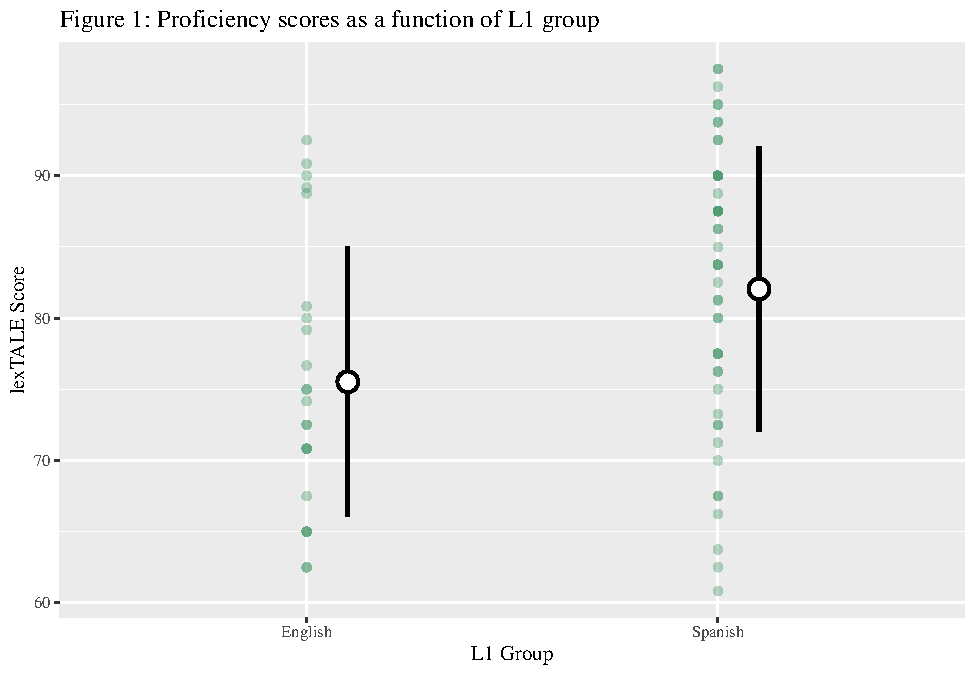
\includegraphics[width=1950px]{master_files/figure-latex/unnamed-chunk-2-1} \caption{Add figure caption here.}\label{fig:unnamed-chunk-2}
\end{figure}

Following these tasks, participants then took a series of three two-alternative forced choice tasks (2afc).
The tasks were programmed in Psychopy (Peirce et al., 2019) and were hosted on Pavlovia.org.
Participants received written instructions prior to taking part in each phase of the experiment. The instructions for the ``English'' task were in English, the instructions for the ``Spanish'' task were in Spanish, and the instructions for the L3 tasks were bilingual (both Spanish and English). In each block, the instructions on profilic were in the language mode that the participants were told that they would hear, and the instructions within the experiment itself were also language specific, with the exception of all L3 prolific instructions being in English. These instructions read ``Final step! You have been assigned to the Hungarian/French group.
The task is the same as the first two sessions, but this time, the words are from the Hungarian/French language.'' In the L3 experimental session, written instructions were more scarce, since the participants had already completed the same procedure twice, but were always presented in both English and Spanish at the same time. Instructions appeared at the beginning of the experiment, after the initial practice trials, and between the stop and vowel sessions, and for the attention checks. In each case, and English instruction was given and its Spanish translation appeared either to the right of the English instruction or immediately below it.
As in previous studies, the instructions contained no instances of the experimental stimuli, in this case ``pafri,'' ``bafri,''ifri, or ``ufri,'' or any of their language specific forms appeared during the instructions.

\hypertarget{stimuli}{%
\subsection{Stimuli}\label{stimuli}}

The 2afc tested the perception of the same two continua (a /p/-/b/ VOT continuum and a /i/-/u/ F2 continuum) in three different language modes: English, Spanish and the L3 (either Hungarian or French). The VOT continuum has been used in previous studies (Gonzales, Byers-Heinlein, \& Lotto, 2019; Lozano-Argüelles et al., 2020) and were created from a recording by a female Spanish-English bilingual. The original VOT continuum contained the word ``pafri'' and ``bafri.'' The recording was resynthesized and ranged in VOT from -35ms to 35ms, excluding a 0 VOT step. In the present study, three additional steps were added on the positive end of the scale in order to increase the chances of /p/ responses at the positive extreme of the continuum, such that steps of 40ms, 45ms, and 50ms were included and made a total of 17 total steps. The extra steps were created manually in PRAAT by extracting 5ms of the voiceless part of the previous segments and adding these portions on to the beginning of the 35ms stimulus up to three times.
Just as in Lozano-Argüelles et al. (2020), the present study conceptually cued participants, and did not utilize the language specific rhotics used in Gonzales and Lotto (2013) and Casillas and Simonet (2018).

The vowel continua were created using productions of the pseudowords ``ifri'' and ``ufri'' by a male American English speaker. These natural productions were then resynthesized using a PRAAT script which manipulated the second formant while holding the other formants constant.
Just as was done with the stop continuum, only the first syllable together with {[}f{]} were produced in each stimulus to avoid perceptual cueing. As a result, the stimuli, ranging from ``if'' to ``uf'' varied only by the second formant (F2: a correlate for frontedness in the vowel space) in a total of 11 steps.

During the 2afc task, participants saw both the words \emph{pafri} and \emph{bafri} or language specific versions of \emph{ifri} and \emph{ufri} on the screen and just the first syllable of these words in which the initial consonant was a member of the continuum (``paf'' or ``baf'' for vowels, ``if'' or ``uf'' for vowels).
Each step of the continuum was played 5 times total, leading to a total of 85 trials in the VOT continuum per participant and 55 total trials in the vowel continuum.
Each trial was drawn randomly from the continuum in a single block, so no participant heard the same stimulus order.
Due to language specific orthographic differences, the non-words on screen were distinct orthographically in each language, with the exception of French and Spanish.
In Spanish and French, the participants saw \emph{ifri} and \emph{ufri} on the screen, in English they saw \emph{eefri} and \emph{oofri}, and in Hungarian, they saw \emph{ifrelo} and \emph{ufrelo}. This spelling difference was necessary because of the orthographic conventions in the realizations of similar sounds between English and Spanish. For example, the Spanish grapheme ``u'' and the English graphemes ``oo'' are similar in their acoustic realizations. On the other hand, the choice of spelling in the French and Hungarian stimuli were made to reflect that high degree of lexical overlap between Spanish and French, and to reinforce the ambiguous relationship between Hungraian and English or Spanish.

\hypertarget{procedure}{%
\subsection{Procedure}\label{procedure}}

<<<<<<< HEAD
All participants completed a total of five tasks, the Language History Questionnaire, the lexTALE proficiency test in their L2, and three 2afc tasks. First, the participants completed the Language History Questionnaire online (Li et al., 2020), followed by the lexTALE proficiency test.
=======
All participants completed a total of five tasks, the Language History Questionnaire, the lexTALE proficiency test in their L2, and three 2afc tasks. First, the participants completed the Language History Questionnaire online (Li, Zhang, Yu, \& Zhao, 2020), followed by the lexTALE proficiency test.
>>>>>>> 0157be86696a9adc7f7de272fdaad6009a47c078
Following these two tasks used for screening, only those participants who did have knowledge of a third language and scored at least 60\% on the lexTALE were deemed eligible and continued the experiment. This cutoff was chosen to focus the analysis on more proficient bilinguals, rather than demonstrate that increasing proficiency is correlated to a larger double phonemic boundary effect size, as has been found in previous studies (Casillas \& Simonet, 2018; Garcia-Sierra, Diehl, \& Champlin, 2009; Gonzales \& Lotto, 2013).

Following these screening tasks, and in order to control for language mode, the participants completed the 2afc tasks in a semi-longitudinal design.
Participants were invited to take part in the second portion of the experiment at least 30 minutes after their completion of the previous step. In many cases, however, participants completed different blocks of the experiment hours or days apart.
All participants began with the ``English'' task, followed by ``Spanish,'' and finished with either ``French'' or ``Hungarian.'' Unfortunately, the lack of counterbalancing across participants is a limitation in the design of the current study.
In the English and Spanish tasks, the instructions were given in that respective language, and it was explained that the participants were going to hear rare words in the language in question (English, Spanish or the L3).
In the L3 session, the same instructions were given in both English and Spanish simultaneously and on the same screen in order to avoid biasing the participants to either English or Spanish mode.

\hypertarget{statistical-analyses}{%
\subsection{Statistical analyses}\label{statistical-analyses}}

In order to determine a crossover boundary for analysis in a general linear model, two logistic regression models were fit to each participant with their responses of `bafri'/`pafri,' in the VOT continuum, and `ifri/ufri,' in the F2 continuum as a function of the standardized continuum step for each language.
The continuum step standardization was done in order to allow for the comparability of the stop and vowel crossover boundaries, which had a distinct number of steps.
As a result, 6 crossover boundaries total were calculated per participant that provided which step in the continuum the probability of the participant choosing either ``pafri'' or ``bafri'' was 50\%. These boundaries were used as continuous variables in subsequent general linear regression models and t-tests. All analyses were carried out in R (R Core Team, 2020) and used either the stats package or the lmer package (Bates, Mächler, Bolker, \& Walker, 2015). In order to determine the independence of the crossover samples, paired t-tests were carried out in each language combination in both stops and vowels. A significant p-value on a paired t-test would indicate that there is non-zero difference between individual participants' crossover boundaries between the two languages.

\hypertarget{results}{%
\section{Results}\label{results}}

\hypertarget{descriptive-statstics}{%
\subsection{Descriptive statstics}\label{descriptive-statstics}}

Tables 2 and 3 provide descriptive statistics of the crossover boundaries per group per language. The crossover boundary is the continuum step at which the probability of choosing both options (/p/ or /b/, or /i/ or /u/) was 50\% and was calculated by fitting a logistic regression model to each participant in each language mode session.
The crossover boundaries were standardized to z-scores in order to allow for comparability across all language modes and over features (between stops and vowels).

\begin{table}[tbp]

\begin{center}
\begin{threeparttable}

\caption{\label{tab:unnamed-chunk-3}Descriptive statistics of vowel crossovers by group}

\begin{tabular}{llllllll}
\toprule
group & \multicolumn{1}{c}{Mean English Crossover} & \multicolumn{1}{c}{SD English} & \multicolumn{1}{c}{Mean Spanish Crossover} & \multicolumn{1}{c}{SD Spanish} & \multicolumn{1}{c}{Mean L3 Crossover} & \multicolumn{1}{c}{SD L3} & \multicolumn{1}{c}{n}\\
\midrule
English\_french & -0.14 & 0.03 & -0.13 & 0.04 & -0.14 & 0.06 & 17\\
English\_hungarian & -0.14 & 0.07 & -0.13 & 0.05 & -0.13 & 0.05 & 17\\
Spanish\_french & -0.07 & 0.05 & -0.11 & 0.06 & -0.10 & 0.06 & 17\\
Spanish\_hungarian & -0.08 & 0.06 & -0.10 & 0.05 & -0.10 & 0.05 & 28\\
\bottomrule
\end{tabular}

\end{threeparttable}
\end{center}

\end{table}

\begin{table}[tbp]

\begin{center}
\begin{threeparttable}

\caption{\label{tab:unnamed-chunk-4}Descriptive statistics of stops crossovers by group}

\begin{tabular}{llllllll}
\toprule
group & \multicolumn{1}{c}{Mean English Crossover} & \multicolumn{1}{c}{SD English} & \multicolumn{1}{c}{Mean Spanish Crossover} & \multicolumn{1}{c}{SD Spanish} & \multicolumn{1}{c}{Mean L3 Crossover} & \multicolumn{1}{c}{SD L3} & \multicolumn{1}{c}{n}\\
\midrule
English\_french & 0.37 & 0.60 & 0.07 & 0.73 & 0.14 & 0.60 & 9\\
English\_hungarian & 0.51 & 0.47 & 0.39 & 0.37 & 0.20 & 0.32 & 14\\
Spanish\_french & -0.14 & 0.74 & -0.30 & 0.50 & -0.27 & 0.46 & 17\\
Spanish\_hungarian & 0.06 & 0.57 & -0.19 & 0.47 & -0.19 & 0.53 & 29\\
\bottomrule
\end{tabular}

\end{threeparttable}
\end{center}

\end{table}

\hypertarget{question-1-was-the-double-phonemic-boundary-effect-replicted-in-stops-and-extended-to-vowels}{%
\subsection{Question 1: Was the double phonemic boundary effect replicted in stops and extended to vowels?}\label{question-1-was-the-double-phonemic-boundary-effect-replicted-in-stops-and-extended-to-vowels}}

In order to answer the research questions of the present study, it was vital to replicate previous findings of double phonemic boundary effect in Spanish-English bilinguals. Thus, an implicit research question in this study was whether Spanish-English bilinguals would show evidence of a double phonemic boundary in stops, as in previous studies, and, newly, whether this effect could be extended to vowels. Of course, without finding two language specific language mode-driven categorizations of English and Spanish, conclusions cannot be drawn as to whether bilinguals approach a third language using their first or second language perceptual routines. The double phonemic boundaries were assessed per language using a series of paired t-tests. The results showed that the English L1 group showed a double phonemic boundary effect in stops (\(t(24) = 2.24\), \(p = .035\)), but not in vowels (\(t(35) = -0.72\), \(p = .477\)). The Spanish L1 group showed evidence of the double phonemic boundary in both stops (\(t(51) = 3.13\), \(p = .003\)) and vowels (\(t(49) = 3.77\), \(p < .001\)). Figure 2 shows a graphical representations of the categorizations of vowels (figure 2) and stops (figure 3) in both languages in both L1 groups.

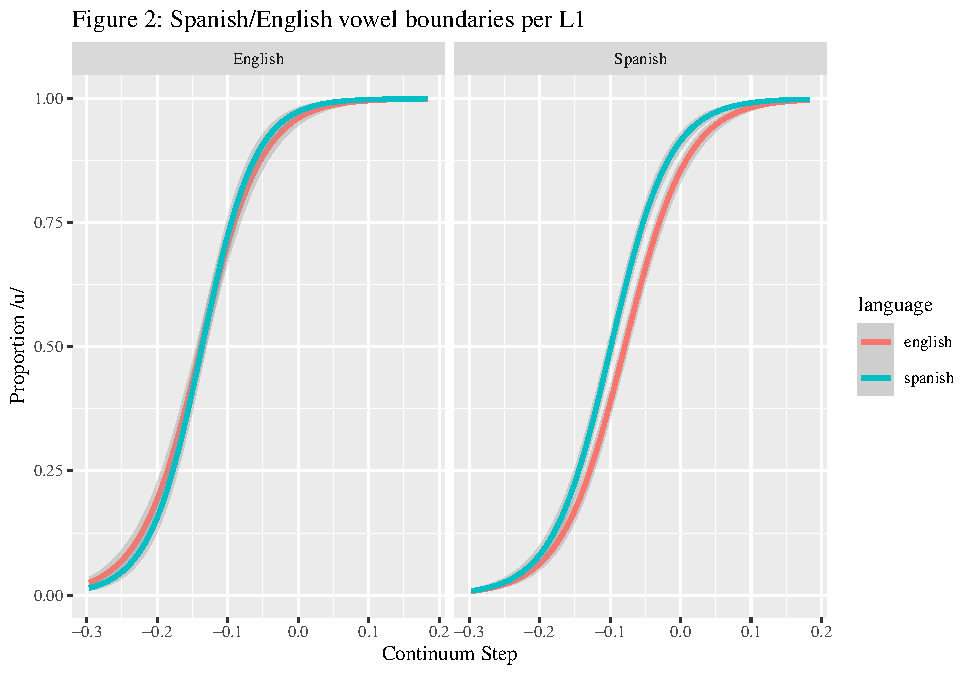
\includegraphics{master_files/figure-latex/unnamed-chunk-5-1.pdf}

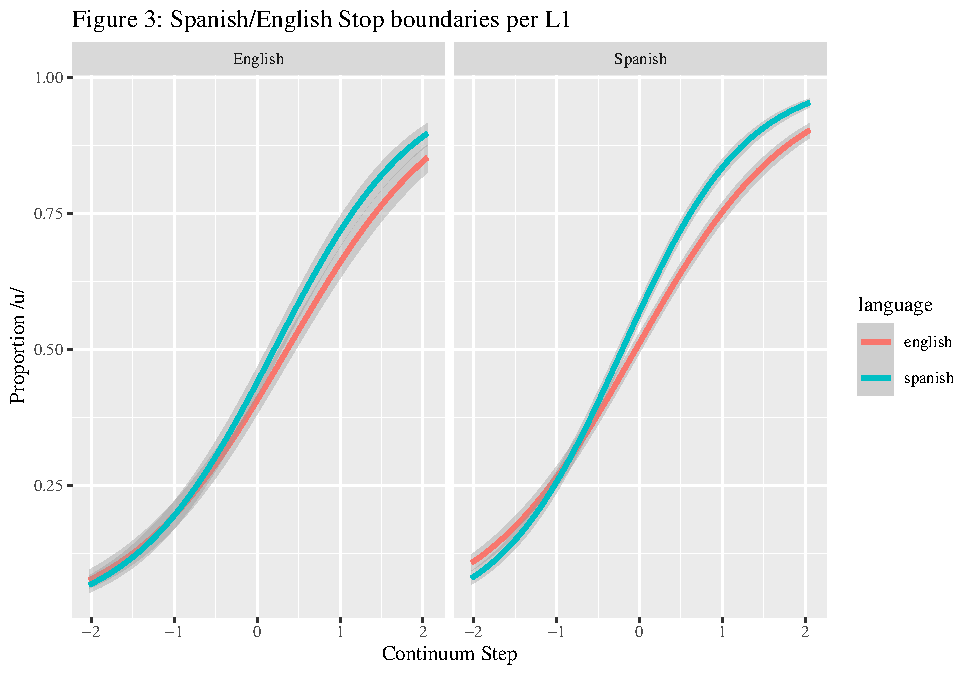
\includegraphics{master_files/figure-latex/unnamed-chunk-6-1.pdf}

\hypertarget{rq2-which-language-specific-phonemic-boundaries-will-participants-perceive-when-they-are-introduced-to-the-same-votf2-continuum-in-a-third-language}{%
\subsection{RQ2: which language-specific phonemic boundaries will participants perceive when they are introduced to the same VOT/F2 continuum in a ``third language?''}\label{rq2-which-language-specific-phonemic-boundaries-will-participants-perceive-when-they-are-introduced-to-the-same-votf2-continuum-in-a-third-language}}

Due to the results of the initial series of paired t-tests, only the results of the stops in both L1 groups and the vowels in the Spanish groups were useful in answering this question, since English vowels violated the necessary assumption that all groups would show double phonemic boundary effects. A series of three paired t-tests are reported per each of the four participant groups. In each group, the paired t-tests serve to provide evidence that language categorizations are independent samples (if the p-value falls below .05) or not independent samples (if the p-value is greater that .05).
The three t-tests in each group test the independence of their L1 and L2 categorization (in all 4 groups), the categorization of their L1 and their L3 (English or Spanish with Hungarian or French), and their L2 and their L3 (also English or Spanish with Hungarian or French). By having all three of the t-tests together, it can more easily be argued that one specific language has greater influence on L3 categorization if, first the Spanish and English paired t-test is significant, and one of the two remaining t-tests is significant and the other is not (i.e.~if the L2 to L3 t-test is significant but the L1 to L3 t-test is not, that is taken as evidence that the L2 and the L3 are independent samples, but that the L1 and the L3 are not).

\hypertarget{stops-english-l1-french-l3-group}{%
\subsubsection{Stops English L1 French L3 group}\label{stops-english-l1-french-l3-group}}

The English L1 group appeared to use their L1 boundary in all three continua in both L1 groups. English L1 vowels did not show a group wide L1-L2 double phonemic boundary effect, and subsequent analyses in the English L1 groups focuses on stops.Despite the group-wide differences in the English L1 group, double phonemic boundary effects were not found in the individual English L1 groups. In stops, paired t-tests found non-significant results, interpreted as similar categorizations in English-Spanish categorization (\(t(8) = 1.48\), \(p = .177\)), Spanish-French categorization (L2 to L3) (\(t(8) = -0.39\), \(p = .706\)) and English-French categorization (L1 to L3) (\(t(8) = 1.14\), \(p = .288\)).

\hypertarget{stops-english-l1-hungarian-l3-group}{%
\subsubsection{Stops English L1 Hungarian L3 group}\label{stops-english-l1-hungarian-l3-group}}

The English-Hungarian stops were found to be distinct. English-Hungarian categorization (L1 to L3) (\(t(13) = 3.02\), \(p = .010\)), but not the English-Spanish categorization (\(t(13) = 1.12\), \(p = .284\)) nor Spanish-Hungarian categorization (L2 to L3) (\(t(13) = 1.77\), \(p = .100\)).

\hypertarget{stops-spanish-l1-french-l3-group}{%
\subsubsection{Stops Spanish L1 French L3 group}\label{stops-spanish-l1-french-l3-group}}

No categorization differences were found in Spanish L1 speakers assigned to the ``French'' group in stops. There was no significant English-Spanish categorization difference (\(t(16) = 0.94\), \(p = .359\)), no significant English-French categorizations difference (\(t(16) = 0.75\), \(p = .467\)) and no significant Spanish-French categorization difference (\(t(16) = -0.50\), \(p = .625\)).

\hypertarget{vowels-spanish-l1-french-l3-group}{%
\subsubsection{Vowels Spanish L1 French L3 group}\label{vowels-spanish-l1-french-l3-group}}

Evidence of a double phonemic Spanish-English boundary was not found in this group (\(t(16) = -0.59\), \(p = .564\)). Likewise, Spanish-French categorizations had no evidence of being distinct (\(t(16) = -0.91\), \(p = .376\)). There was, however, evidence of a distinction in English-French categorizations (\(t(16) = 3.20\), \(p = .006\)). The lack of evidence for the double phonemic boundary effect in this group alone does not allow for definitive evidence that can inform which language boundary this group used in the perception of what they believed were French vowels.

\hypertarget{stops-spanish-l1-hungarian-l3-group}{%
\subsubsection{Stops Spanish L1 Hungarian L3 group}\label{stops-spanish-l1-hungarian-l3-group}}

In this group, there was evidence that there was a English-Spanish categorization difference (\(t(28) = 2.80\), \(p = .009\)), implying that this group showed evidence of the double phonemic boundary. The L2 and L3 English-Hungarian categorizations were also found to be categorized differently (\(t(28) = 2.47\), \(p = .020\)), whereas the L1 and the L3 Spanish-Hungarian categorizations (\(t(28) = -0.10\), \(p = .922\)) were not categorized differently.
These results suggest that the Spanish L1 group used their L1 boundaries to categorize what they believed were Hungarian stops.

\hypertarget{vowels-spanish-l1-hungarian-l3-group}{%
\subsubsection{Vowels Spanish L1 Hungarian L3 group}\label{vowels-spanish-l1-hungarian-l3-group}}

The same trend is present in vowels as in stops for the Spanish L1 Hungarian L3 group. A paired t-test examining the cross over boundaries of English and Spanish (\(t(27) = 2.08\), \(p = .048\)) reveals a double phonemic boundary effect. There was evidence that there is a difference in L2-L3 English-Hungarian categorizations (\(t(27) = 2.20\), \(p = .037\)), but another paired t-test suggests that L1-L3 Spanish-Hungarian (\(t(27) = 0.23\), \(p = .818\)) are not categorized distinctly. Like stops, taken together, these results suggest that the Spanish L1 group used their L1 boundaries to categorize what they believed were Hungarian vowels.

\hypertarget{rq3-did-the-l3-groups-categorize-the-continua-differently}{%
\subsection{RQ3: Did the L3 groups categorize the continua differently?}\label{rq3-did-the-l3-groups-categorize-the-continua-differently}}

T-tests of independent samples revealed that L3 groups did not categorize their respective continua differently if they were assigned to the French group or the Hungarian group. The L3 French group with Spanish L1 and the L3 Hungarian group with a Spanish L1 did not categorize their respective L3s differently in vowels (\(t(31.25) = 0.10\), \(p = .924\)) or stops (\(t(37.81) = 0.55\), \(p = .585\)). The same evidence was found the the English L1 groups; they categorized L3 sounds similarly, whether they were in the L3 French group or Hungarian group in both vowels (\(t(29.90) = 0.57\), \(p = .573\)) and stops (\(t(10.89) = 0.28\), \(p = .788\)).

\hypertarget{post-hoc-analysis}{%
\subsection{Post-hoc analysis}\label{post-hoc-analysis}}

Based on the findings that the suggested that L3 continua were not categorized differently by the same L1 group, a post-hoc series of paired tests of equivalence were carried out in which the L3 groups were pooled together.
First, tests of equivalence were carried out to determine whether L3 groups categorized the continua equivalently whether they believed the were hearing Hungarian or French.
Importantly, the same participants did not hear both French and Hungarian, but were randomly assigned to one of them. As a result, a non-paired test of equivalence was carried out. Cohen's D was set to .5 in these tests, which has been reported as a medium effect size in the literature (Cohen, 2013).
All tests were carried out in R (R Core Team, 2020), using the \texttt{TOSTER} function (Lakens, 2017).

Figure 4 shows a graphical summary of three non-paired tests of equivalence. The first was a comparison between categorization of vowels between the French L3 and Hungarian L3 groups with Spanish as their L1. Surprisingly, the equivalence test was did not quite show that the categorizations of French and Hungarian vowels by the Spanish L1 groups were equivalent (t(31.25) = -1.510, p = 0.0705, given equivalence bounds of -0.0266 and 0.0266 (on a raw scale) and an alpha of 0.05).
It is likely that, it this case, the lack of equivalence found is due to a low sample size.

The second test of equivalence measured the categorizations of stops between the French and Hungarian L3 groups who speak L1 Spanish. These results are similar to those reported in vowels in that they do not provide enough evidence that the L3 groups categorized what they believed to be L3 sounds the same (t(37.81) = -1.118, p = 0.135, given equivalence bounds of -0.248 and 0.248 (on a raw scale) and an alpha of 0.05).
Again, this is suggested to be due to low sample size.

The third test of equivalence measured the categorizations of stops between the French and Hungarian L3 groups who speak L1 English. A similar trend was observed in this case, in which equivalence was not detected, likely due to low sample size (t(10.89) = -0.829, p = 0.212, given equivalence bounds of -0.242 and 0.242 (on a raw scale) and an alpha of 0.05.).

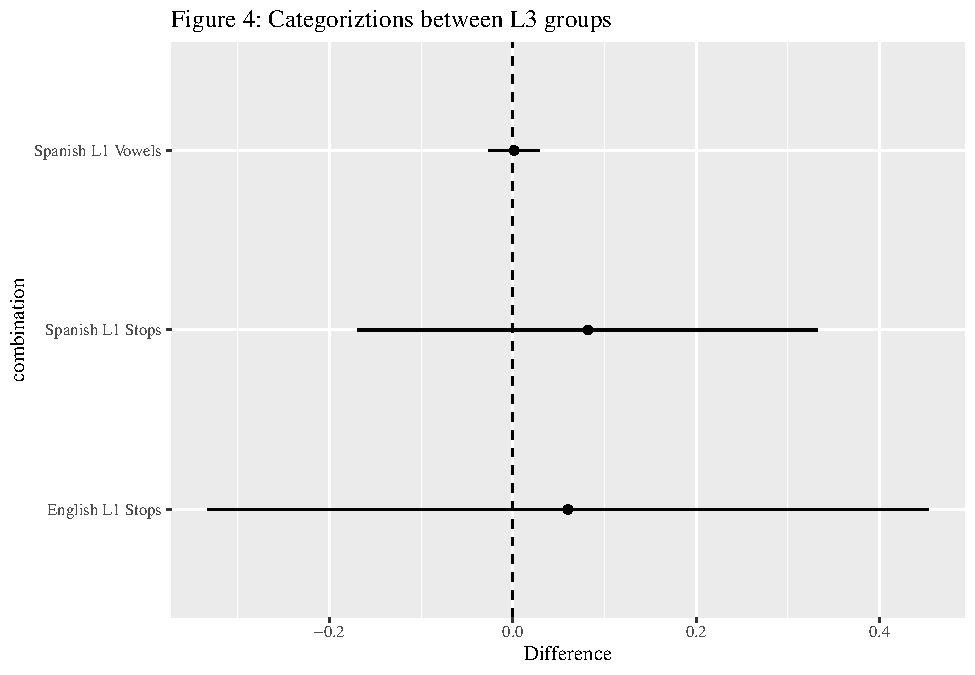
\includegraphics{master_files/figure-latex/unnamed-chunk-7-1.pdf}

Inspired by the idea that low sample size may be the cause of the lack of equivalence in the findings, an additional series of paired equivalence tests were carried out in Spanish L1 vowels, Spanish L1 stops, and English L1 stops. English L1 vowels were omitted due to the lack of any recognizable trend towards a meaningful difference in the initial analysis.

\hypertarget{spanish-l1-group-pooled-stops}{%
\subsubsection{Spanish L1 group pooled stops}\label{spanish-l1-group-pooled-stops}}

Firstly, this group showed evidence of the double phonemic boundary effect when they were pooled (\(t(45) = 2.62\), \(p = .012\)).
Next, of interest in this group was whether the Spanish L1 group categorized the L3 stop continua using their L1 boundaries. The test of equivalence suggest that this is the case (t(45) = -3.094, p = 0.00169).
On the other hand, English and the L3 were not found to be equivalent (t(45) = -1.103, p = 0.138), and nor were Spanish and English (t(45) = -0.770, p = 0.223).
Figures 5 is a graphical representation of the crossover boundaries of stops in the pooled data of both Spanish L1 groups.
Figure 6 shows the effect sizes derived from each of the three tests of equivalence.
As can be seen in figure 6, the smallest effect size is the difference between the L1 and the L3, which is rather close to zero.

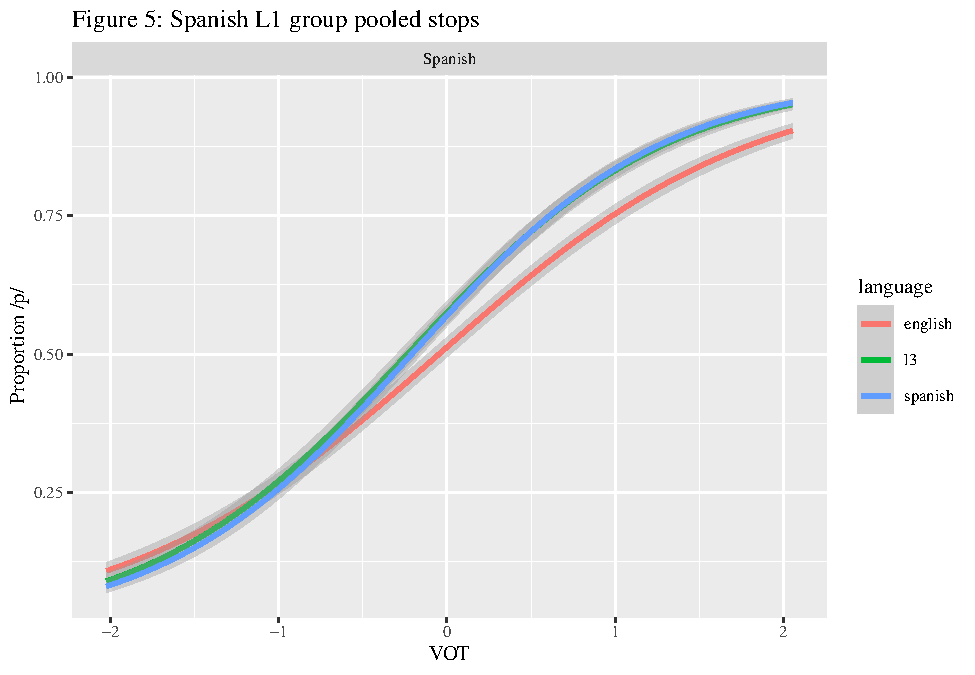
\includegraphics{master_files/figure-latex/unnamed-chunk-8-1.pdf} 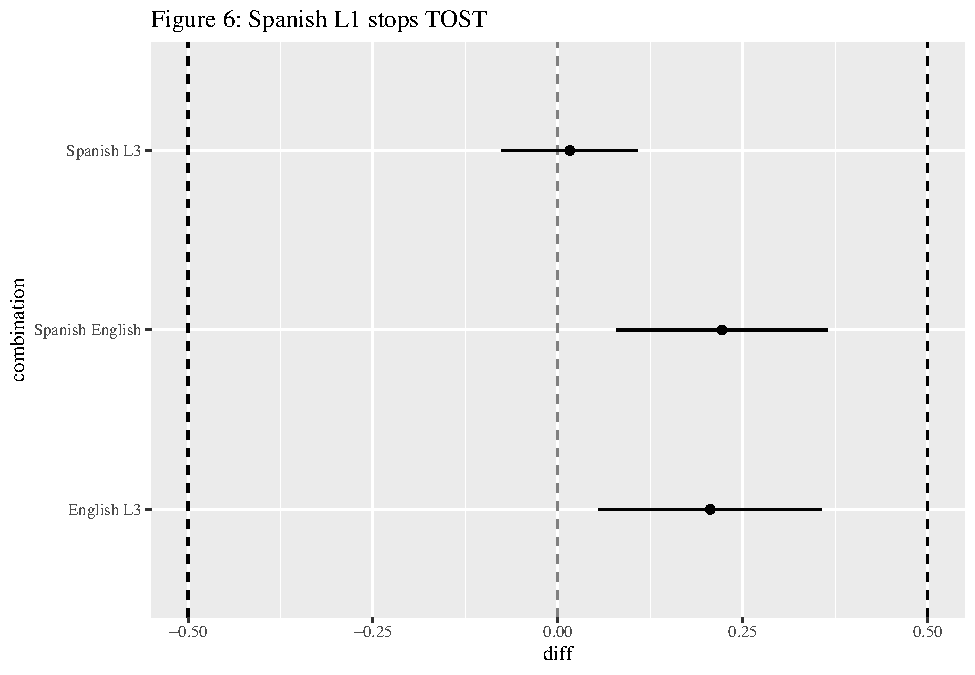
\includegraphics{master_files/figure-latex/unnamed-chunk-8-2.pdf}

\hypertarget{spanish-l1-group-pooled-vowels}{%
\subsubsection{Spanish L1 group pooled vowels}\label{spanish-l1-group-pooled-vowels}}

A similar results was found in the Spanish L1 group in vowels. First, there was evidence of a double phonemic boundary (\(t(44) = 3.88\), \(p < .001\)) between English and Spanish.
Next, there is evidence that the L1 and the L3 were categorized equivalently (t(45) = -2.949, p = 0.00252), where the L2 and L3 (t(45) = 0.198, p = 0.578) and the L1 and the L2 (t(45) = 0.536, p = 0.703) were not.
Just as in stops, Figure 7 is a graphical representation of the crossover boundaries of vowels in the pooled data of both Spanish L1 groups.
Figure 8 shows the effect sizes derived from each of the three tests of equivalence.
Again, similarly to stops, in figure 8, the smallest effect size is the difference between the L1 and the L3, which is rather close to zero.

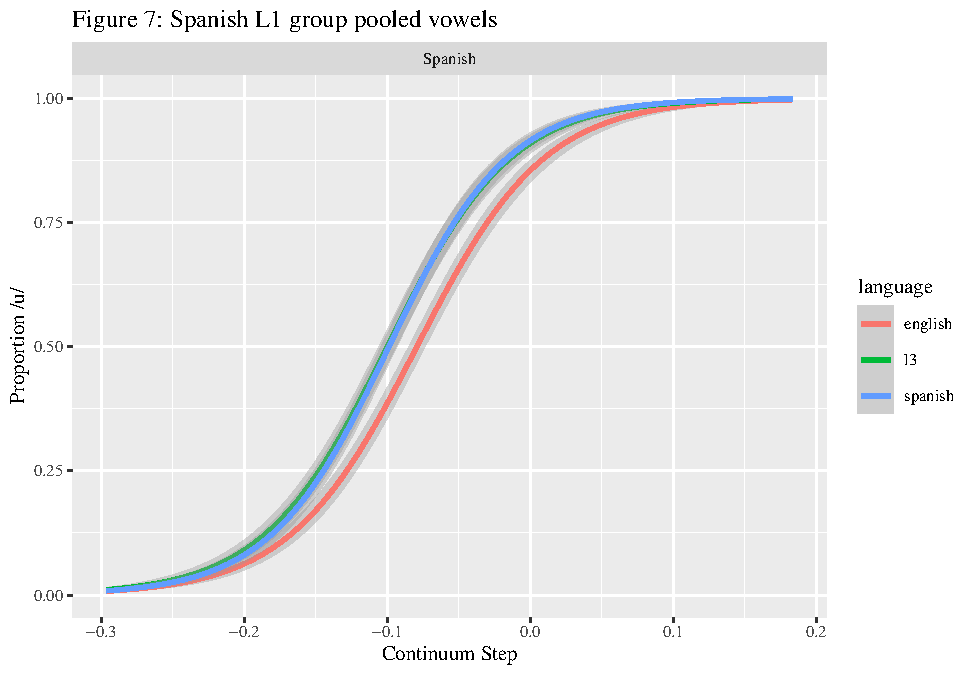
\includegraphics{master_files/figure-latex/unnamed-chunk-9-1.pdf} 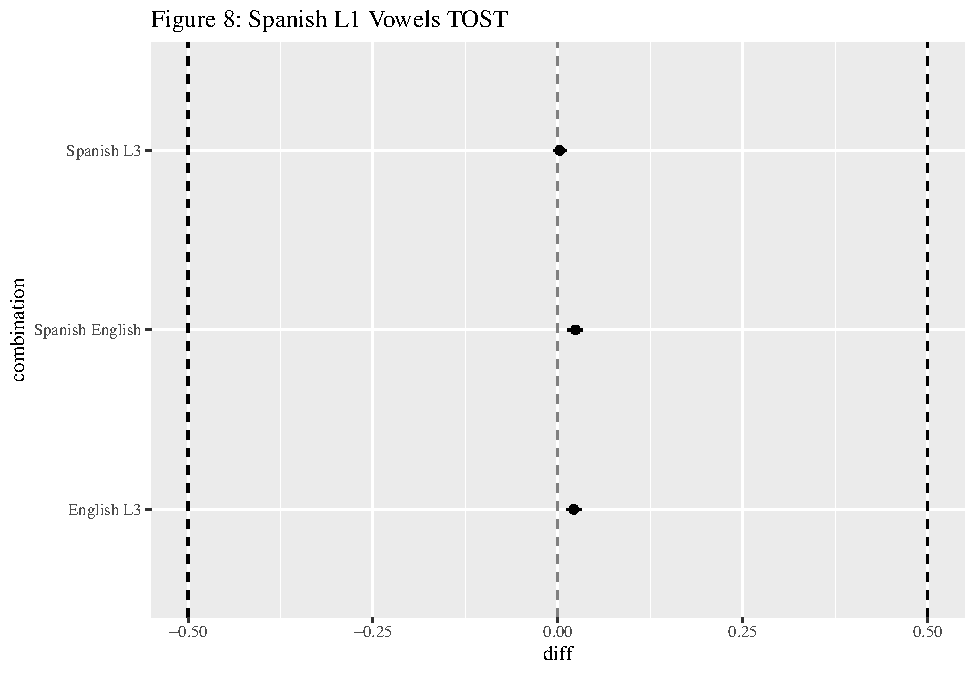
\includegraphics{master_files/figure-latex/unnamed-chunk-9-2.pdf}

\hypertarget{english-l1-group-pooled-stops}{%
\subsubsection{English L1 group pooled stops}\label{english-l1-group-pooled-stops}}

Overall, clear conclusions cannot be drawn regarding the English L1 group's categorization of stops.
In the fist analysis, only the stops showed evidence of a double phonemic boundary modulated by language mode, however, this Spanish-English double phonemic boundary effect does not quite persist in those who completed all phases of the experiment (\(t(22) = 1.87\), \(p = .075\)).

The data also suggested that this group showed evidence of their L2 influencing L3 comprehension, rather than their L1. The equivalence test between L2 and L3 was the closest to equivalent, t(22) = 1.441, p = 0.0818), but did not provide sufficient evidence to classify the data as evidence for an L2 status effect.
Importantly, this groups L1 and L3 categorizations were not equivalent (t(22) = 0.427, p = 0.663), and neither were their L1 and L2 categorizations (t(22) = -0.527, p = 0.302)
Just as in the previously reported tests of equivalence, figures 9 shows the graphical representation of the crossover boundaries of stops in the pooled data of both English L1 groups.
Figure 10 shows the relative effect sizes of each language combination.
Taken together, it is difficult to draw clear conclusions in regard to the English L1 group.

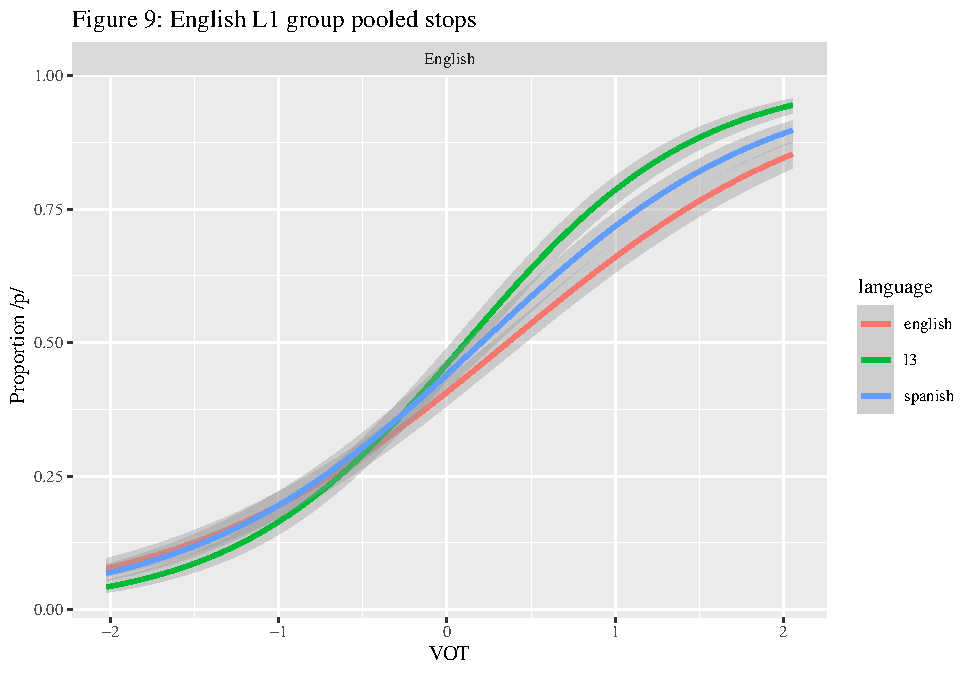
\includegraphics{master_files/figure-latex/unnamed-chunk-10-1.pdf} 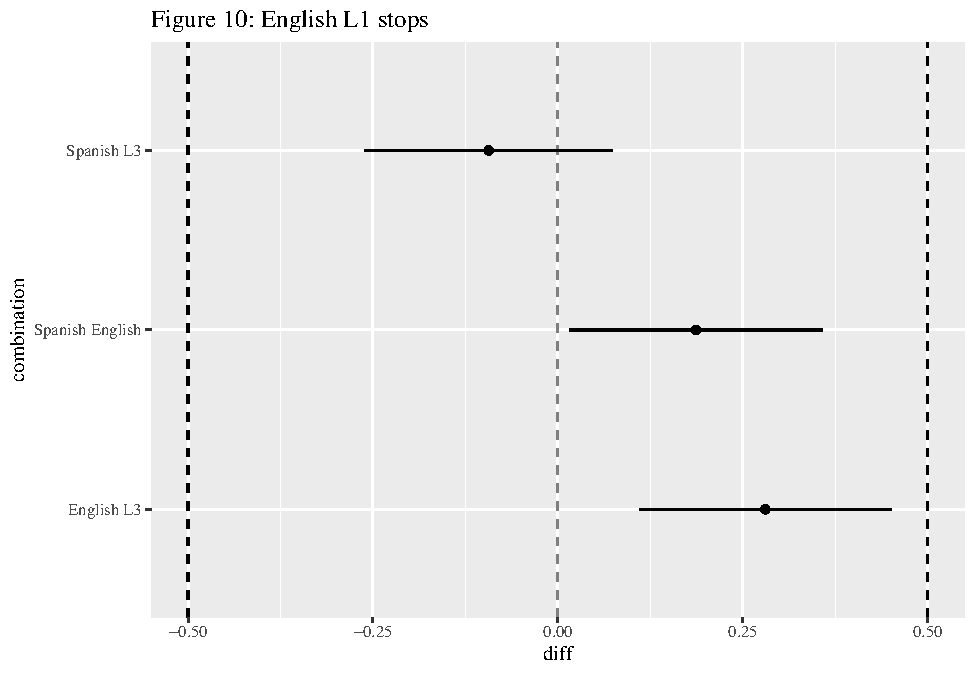
\includegraphics{master_files/figure-latex/unnamed-chunk-10-2.pdf}

<<<<<<< HEAD
=======
\hypertarget{discussion}{%
\section{Discussion}\label{discussion}}

\hypertarget{summary-of-findings}{%
\subsection{Summary of findings}\label{summary-of-findings}}

The present study attempted to replicate the double phonemic boundary effect in adult Spanish-English bilinguals in both orders of acquisition in two continua, a voicing continuum, and a vowel continuum, in order to investigate how language specific categorization of the continua interacted with a third language at first exposure that the participants did not know, either French or Hungarian. The results showed evidence of L1 influence on L3 categorizations in the Spanish L1 group. This L1 effect was seen in both Spanish L1 L3 groups and in stops and vowels, and was observed in both the French and Hungarian L3 groups. Additionally, the results also showed evidence of L2 influence on L3 categorizations of stops in the English L1 group, but not vowels. Overall, the English L1 group did not show evidence of language specific vowel categorizations. Finally, the present study replicated the findings of a double phonemic boundary effect found in previous studies (Casillas \& Simonet, 2018; Gonzales \& Lotto, 2013; Lozano-Argüelles et al., 2020) in both Spanish L1 bilinguals and English L1 bilinguals, and extended the double phonemic boundary to vowels in the Spanish L1 group.

\hypertarget{revisiting-the-predictions-of-l3-models}{%
\subsection{Revisiting the predictions of L3 models}\label{revisiting-the-predictions-of-l3-models}}

Taken together, the results of the present study cannot be explained by any of the L3 models of morphosyntax alone. The TPM predicted that one language would holistically transfer to the L3, and could be either the L1 or the L2, but not features of both languages.
The English L1 group provides counter-evidence to this prediction, since they categorized the stop continuum similarly to their L2 categorization, and did not have language distinct categorizations in the vowel continuum. In the view of the TPM, but continua should have been influenced by the same language, rather than the L3 stops being categorized using L1 perceptual boundaries and vowels being categorized using L2 perceptual boundaries. This case was arguably observed in the English L1 group, who categorized vowels similarly in all 3 language contexts, but categorized the L3 stops as similar to their L2.

Additionally, it was expected that the French and Hungarian L3 groups would categorize their L3 differently. In the case of the French group, I predicted that both groups would be biased towards categorizing the L3 continua similarly to their Spanish continua, regardless of their order of acquisition.
This prediction was based on previous findings in support of the TPM, in which typological transfer was found in language combinations that contained two romance languages and English (with many studies examining Brazilian Portuguese as the L3 in Spanish-English bilinguals).
Similar evidence has yet to be observed in other language groupings, in which the L1 and the L2 of two different groups (that are the same language) serve as the basis of influence to the L3. This result is conceived of as evidence of typological transfer by the TPM (in the case of syntax).
Following this lack of cross-linguistic support for the TPM, the Hungarian group was included in the present study, to see whether participant's belief that they were listening to French or Hungarian would differ.
The predictions of the default source of influence to the Hungarian group's categorizations is much less straightforward than the predictions of the French group.
In this case, in which there is not a relatively clear typological relationship between two out of three languages in the L3 learner, the literature supports the prediction of L2 status effects by default, meaning that the L2 of the participant would be the source of influence on their L3 categorizations.

The results of the present study did not confirm either of these predictions. The French and Hungarian groups did not categorize the continua differently in either L1 group.
In terms of L2 status, the English L1 group showed L2 influence in their categorization of L3 stops in both French and Hungarian, but not in vowels. The result that the English L1 group did not categorize both stops and vowels as similar to the same source of influence (i.e.~the L1 or the L2) is incompatible with full transfer models, the TPM and the L2SF.
In a sense, the LPM can account for this difference, but cannot be said to have predicted it, since the model does not specify clear criteria for when influence does and does not occur.

\hypertarget{comparisons-to-previous-language-set-studies}{%
\subsection{Comparisons to previous language set studies}\label{comparisons-to-previous-language-set-studies}}

The present study was successful in replicating the result of previous studies which found a double phonemic boundary effect in bilinguals (Casillas \& Simonet, 2018; Gonzales, Byers-Heinlein, \& Lotto, 2019; Gonzales \& Lotto, 2013; Lozano-Argüelles et al., 2020). In addition to replication, the result of the present study show that it is possible that both L1 Spanish speakers who learn English and L1 English speakers who learn Spanish both have language specific categorizations of sounds based on language context. This effect was found in both groups for stops, and was extended to the vowel continuum in the Spanish L1 group. The English L1 group, on the other hand, did not categorize the vowel continuum differently when they were led to believe that they were hearing English, Spanish or a L3.
The present study used conceptual cueing, as done in Gonzales, Byers-Heinlein, and Lotto (2019) and Lozano-Argüelles et al. (2020) , rather than perceptual cueing, to mitigate the possible effect of cross-language segmental similarity biasing perception. As as result, the present study provides a third replication of conceptual cueing in Spanish-English bilinguals in stops.

On the other hand, it is unclear why the English L1 group did not categorize the vowel continuum distinctly based on language mode. It is possible that the English L1 group has not established stable L2 vowel categories, due to their lower proficiency relative to the Spanish L1 group. On the other hand, it is possible that /u/ fronting in some dialects of English may have biased the results of this group in vowels to have categorized a large part of the continuum in the present study as /u/. Likewise, the context of the experiments between groups could not be carefully and completely controlled due to the challenges of online data collection during the COVID era. It is possible that the English speaking group was simply not as sensitive to the instructions when being biased towards a particular language mode. It is worth noting that the website used for prolific is a British based company, and that the participants using this site may approach it in a default English mode. It is possible that the instructions alone were not a strong enough manipulation to break these participants completely from an English mode. It is worth noting, however that the same participants did categorize the stop continuum differently based on language mode, further complicating the issue. The continua were distinct in that the vowel continuum was produced by a male speaker and the stop continuum was produced by a female speaker. As a result, the average pitch of the vowel continuum was likely lower than the stop continuum. It could be that the English speaking group was sensitive to this pitch difference, where the Spanish group was not.

\hypertarget{limitations-and-furture-research}{%
\subsection{Limitations and Furture Research}\label{limitations-and-furture-research}}

These mixed results also may have been caused by the limitations of the present study. A study conducted online likely cannot control for headphones, and the different sound quality among participants' headphones cannot be well controlled for, not ruled out as a possible influence in the results. Likewise, without researcher supervision, participant effort cannot be well evaluated. In the case of the present study, it is unclear whether some participants did no perceive a difference in the steps on the continua due to their phonology or they wanted to complete the experiment as quickly as possible and did not give a genuine effort. Finally, the present study did not control for geographical separation and dialectal variation. The English L1 group contains native speakers of English world wide, including American, British English, and Irish English speakers. The Spanish L1 group, on the other hand, consists of speakers from mostly Mexico, Spain, and Chile. These challenges, together with the low sample size of the present study, suggest that the results reported here be interpreted with caution.

Future research should consider more carefully the effects of context in online data collection, should this style of data collection continue to be necessary. Limiting a group of participants geographically is vital, since dialectal variation may impact results. In addition, attention checks are helpful for avoiding low effort submissions.

Theoretically, the evidence from the present study highlights the need to L3 phonology specific studies and models, and the need to carry out experiments in perception and production. The results reported here run contrary to those in production reported in the L3 phonology literature, such as (B. Hammarberg \& Hammarberg, 1993), in which the authors found a global influence of L2 in the beginning of L3 acquisition that eventually was replaced by L1 influence at a later testing time.
Here, evidence of L2 influence was only found in the English L1 group in stops, while the Spanish L1 group showed evidence of L1 influence on L3 categorizations.
Further studies are needed to determine whether this asymmetry in production and perception will hold up cross-linguistically, and within the same participants.
Additionally, given the lack of accurate predictions by L3 models of morphosyntax in L3 perception, further study is needed to determine the factors which influence cross-linguistic influence in L3 perception.

\hypertarget{conclusion}{%
\section{Conclusion}\label{conclusion}}

The present study replicated the findings of previous studies that found evidence of conceptually-cued language mode effects in sound categorizations in late bilinguals (Gonzales, Byers-Heinlein, \& Lotto, 2019; Lozano-Argüelles et al., 2020) and, in an extension to previous studies, found evidence of a double phonemic boundary effect in vowels.
The predictions of L3 models of morphosyntax were not supported by the evidence of the present study. In particular, the predominant trend in L3 perception was a default L1 influence in the Spanish L1 group, but was the opposite in the English L1 group, where an L2 influence was observed in stops only.
This L1 influence persisted in both stops and vowels in the Spanish L1 group, and does not support the predictions of any of the L3 models tested here. Moving forward, a model for L3 phonology is likely needed, which should examine and predict both production and perception.

>>>>>>> 0157be86696a9adc7f7de272fdaad6009a47c078
\hypertarget{references}{%
\section{References}\label{references}}

\begingroup
\setlength{\parindent}{-0.5in}
\setlength{\leftskip}{0.5in}

\hypertarget{refs}{}
\begin{CSLReferences}{1}{0}
<<<<<<< HEAD
\leavevmode\vadjust pre{\hypertarget{ref-R-lme4}{}}%
Bates, D., Mächler, M., Bolker, B., \& Walker, S. (2015). Fitting linear mixed-effects models using {lme4}. \emph{Journal of Statistical Software}, \emph{67}(1), 1--48. \url{https://doi.org/10.18637/jss.v067.i01}

\leavevmode\vadjust pre{\hypertarget{ref-casillas_perceptual_2018}{}}%
Casillas, J. V., \& Simonet, M. (2018). Perceptual categorization and bilingual language modes: Assessing the double phonemic boundary in early and late bilinguals. \emph{Journal of Phonetics}, \emph{71}, 51--64. \url{https://doi.org/10.1016/j.wocn.2018.07.002}

\leavevmode\vadjust pre{\hypertarget{ref-cohen_statistical_2013}{}}%
Cohen, J. (2013). \emph{Statistical power analysis for the behavioral sciences.} Burlington: Elsevier Science. Retrieved from \url{https://search.ebscohost.com/login.aspx?direct=true\&scope=site\&db=nlebk\&db=nlabk\&AN=923159}

\leavevmode\vadjust pre{\hypertarget{ref-garcia-sierra_testing_2009}{}}%
Garcia-Sierra, A., Diehl, R. L., \& Champlin, C. (2009). Testing the double phonemic boundary in bilinguals. \emph{Speech Communication}, \emph{51}(4), 369--378. \url{https://doi.org/10.1016/j.specom.2008.11.005}

\leavevmode\vadjust pre{\hypertarget{ref-gonzales_how_2019}{}}%
Gonzales, K., Byers-Heinlein, K., \& Lotto, A. J. (2019). How bilinguals perceive speech depends on which language they think they're hearing. \emph{Cognition}, \emph{182}, 318--330.

\leavevmode\vadjust pre{\hypertarget{ref-gonzales_bafri_2013}{}}%
Gonzales, K., \& Lotto, A. J. (2013). A \emph{bafri} , un \emph{pafri}: Bilinguals' pseudoword identifications support language-specific phonetic systems. \emph{Psychological Science}, \emph{24}(11), 2135--2142. \url{https://doi.org/10.1177/0956797613486485}

\leavevmode\vadjust pre{\hypertarget{ref-izura_lexical_2016}{}}%
Izura, C., Cuetos, F., \& Brysbaert, M. (2016). \emph{Lexical test for advanced learners of spanish}. American Psychological Association. \url{https://doi.org/10.1037/t47086-000}

\leavevmode\vadjust pre{\hypertarget{ref-toster}{}}%
Lakens, D. (2017). Equivalence tests: A practical primer for t-tests, correlations, and meta-analyses. \emph{Social Psychological and Personality Science}, \emph{1}, 1--8. \url{https://doi.org/10.1177/1948550617697177}

\leavevmode\vadjust pre{\hypertarget{ref-lemhofer_lexical_2016}{}}%
Lemhöfer, K., \& Broersma, M. (2016). \emph{Lexical test for advanced learners of english}. American Psychological Association. \url{https://doi.org/10.1037/t47085-000}

\leavevmode\vadjust pre{\hypertarget{ref-li_language_2020}{}}%
Li, P., Zhang, F., Yu, A., \& Zhao, X. (2020). Language history questionnaire ({LHQ}3): An enhanced tool for assessing multilingual experience. \emph{Bilingualism: Language and Cognition}, \emph{23}(5), 938--944. \url{https://doi.org/10.1017/S1366728918001153}

\leavevmode\vadjust pre{\hypertarget{ref-lozano-arguelles_conceptually_2020}{}}%
Lozano-Argüelles, C., Fernández Arroyo, L., Rodríguez, N., Durand López, E. M., Garrido Pozú, J. J., Markovits, J., \ldots{} Casillas, J. V. (2020). {CONCEPTUALLY} {CUED} {PERCEPTUAL} {CATEGORIZATION} {IN} {ADULT} L2 {LEARNERS}. \emph{Studies in Second Language Acquisition}, 1--16. \url{https://doi.org/10.1017/S0272263120000273}

\leavevmode\vadjust pre{\hypertarget{ref-peirce_psychopy2_2019}{}}%
Peirce, J., Gray, J. R., Simpson, S., MacAskill, M., Höchenberger, R., Sogo, H., \ldots{} Lindeløv, J. K. (2019). {PsychoPy}2: Experiments in behavior made easy. \emph{Behavior Research Methods}, \emph{51}(1), 195--203. \url{https://doi.org/10.3758/s13428-018-01193-y}

\leavevmode\vadjust pre{\hypertarget{ref-R-base}{}}%
R Core Team. (2020). \emph{R: A language and environment for statistical computing}. Vienna, Austria: R Foundation for Statistical Computing. Retrieved from \url{https://www.R-project.org/}

=======
\leavevmode\hypertarget{ref-abbes_acquisition_2016}{}%
Abbes, K. B. (2016). \emph{The acquisition of french morpho-syntactic properties: Cross-linguistic influence in the learning of L3 french by turkish/spanish speakers who learned english as an L2}. \url{https://doi.org/10.13140/RG.2.2.35972.78726}

\leavevmode\hypertarget{ref-balas_perception_2019}{}%
Balas, A., Kopečková, R., \& Wrembel, M. (2019). {PERCEPTION} {OF} {RHOTICS} {BY} {MULTILINGUAL} {CHILDREN}. In S. Calhoun, P. Escudero, M. Tabain, \& P. Warren (Eds.), \emph{Proceedings of the 19th international congress of phonetic sciences}. Melbourne, Australia: Canberra, Australia: Australasian Speech Science; Technology Association Inc.

\leavevmode\hypertarget{ref-bardel_role_2007}{}%
Bardel, C., \& Falk, Y. (2007). The role of the second language in third language acquisition: The case of germanic syntax. \emph{Second Language Research}, \emph{23}(4), 459--484. \url{https://doi.org/10.1177/0267658307080557}

\leavevmode\hypertarget{ref-cabrelli_amaro_l2_2012}{}%
Bardel, C., \& Falk, Y. (2012). The L2 status factor and the declarative/procedural distinction. In J. Cabrelli Amaro, S. Flynn, \& J. Rothman (Eds.), \emph{Studies in bilingualism} (Vol. 46, pp. 61--78). Amsterdam: John Benjamins Publishing Company. \url{https://doi.org/10.1075/sibil.46.06bar}

\leavevmode\hypertarget{ref-bardel_l1_2020}{}%
Bardel, C., \& Falk, Y. (2020). L1, L2 and L3: Same or different? \emph{Second Language Research}, 026765832094103. \url{https://doi.org/10.1177/0267658320941033}

\leavevmode\hypertarget{ref-R-lme4}{}%
Bates, D., Mächler, M., Bolker, B., \& Walker, S. (2015). Fitting linear mixed-effects models using {lme4}. \emph{Journal of Statistical Software}, \emph{67}(1), 1--48. \url{https://doi.org/10.18637/jss.v067.i01}

\leavevmode\hypertarget{ref-blank_transferencia_2009}{}%
Blank, C. A., \& Zimmer, M. C. (2009). A transferência fonético-fonológica L2 (francês) -- L3 (inglês): Um estudo de caso. \emph{Revista de Estudos Da Linguagem}, \emph{17}(1), 207--233. \url{https://doi.org/10.17851/2237-2083.17.1.207-233}

\leavevmode\hypertarget{ref-borg_acquisition_2013}{}%
Borg, K. (2013). The acquisition of future of probability in L3 spanish. \emph{Proceedings of the 12th generative approaches to second language acquisition}. Presented at the {GALSA}.

\leavevmode\hypertarget{ref-bruhn_de_garavito_subject_2014}{}%
Bruhn de Garavito, J., \& Perpiñán, S. (2014). Subject pronouns and clitics in the spanish interlanguage of french L1 speakers. \emph{Subject pronouns and clitics in the spanish interlanguage of french L1 speakers}. Presented at the Canadian linguistic association conference proceedings.

\leavevmode\hypertarget{ref-peukert_relationship_2015}{}%
Cabrelli Amaro, J., Felipe Amaro, J., \& Rothman, J. (2015). The relationship between L3 transfer and structural similarity across development: Raising across an experiencer in brazilian portuguese. In H. Peukert (Ed.), \emph{Hamburg studies on linguistic diversity} (Vol. 4, pp. 21--52). Amsterdam: John Benjamins Publishing Company. \url{https://doi.org/10.1075/hsld.4.02ama}

\leavevmode\hypertarget{ref-cabrelli_amaro_investigating_2016}{}%
Cabrelli Amaro, J., \& Wrembel, M. (2016). Investigating the acquisition of phonology in a third language -- a state of the science and an outlook for the future. \emph{International Journal of Multilingualism}, \emph{13}(4), 395--409. \url{https://doi.org/10.1080/14790718.2016.1217601}

\leavevmode\hypertarget{ref-caramazza_acquisition_1973}{}%
Caramazza, A., Yeni‐Komshian, G. H., Zurif, E. B., \& Carbone, E. (1973). The acquisition of a new phonological contrast: The case of stop consonants in french‐english bilinguals. \emph{The Journal of the Acoustical Society of America}, \emph{54}(2), 421--428. \url{https://doi.org/10.1121/1.1913594}

\leavevmode\hypertarget{ref-caramazza_voice_1974}{}%
Caramazza, A., \& Yeni-Komshian, G. H. (1974). Voice onset time in two french dialects. \emph{Journal of Phonetics}, \emph{2}(3), 239--245. \url{https://doi.org/10.1016/S0095-4470(19)31274-4}

\leavevmode\hypertarget{ref-caramazza_bilingual_1974}{}%
Caramazza, A., Yeni-Komshian, G., \& Zurif, E. B. (1974). Bilingual switching: The phonological level. \emph{Canadian Journal of Psychology/Revue Canadienne de Psychologie}, \emph{28}(3), 310--318. \url{https://doi.org/10.1037/h0081997}

\leavevmode\hypertarget{ref-casillas_perceptual_2018}{}%
Casillas, J. V., \& Simonet, M. (2018). Perceptual categorization and bilingual language modes: Assessing the double phonemic boundary in early and late bilinguals. \emph{Journal of Phonetics}, \emph{71}, 51--64. \url{https://doi.org/10.1016/j.wocn.2018.07.002}

\leavevmode\hypertarget{ref-cohen_statistical_2013}{}%
Cohen, J. (2013). \emph{Statistical power analysis for the behavioral sciences.} Burlington: Elsevier Science. Retrieved from \url{https://search.ebscohost.com/login.aspx?direct=true\&scope=site\&db=nlebk\&db=nlabk\&AN=923159}

\leavevmode\hypertarget{ref-elman_perceptual_1977}{}%
Elman, J. L., Diehl, R. L., \& Buchwald, S. E. (1977). Perceptual switching in bilinguals. \emph{The Journal of the Acoustical Society of America}, \emph{62}(4), 971--974. \url{https://doi.org/10.1121/1.381591}

\leavevmode\hypertarget{ref-falk_role_2015}{}%
Falk, Y., Lindqvist, C., \& Bardel, C. (2015). The role of L1 explicit metalinguistic knowledge in L3 oral production at the initial state. \emph{Bilingualism: Language and Cognition}, \emph{18}(2), 227--235. \url{https://doi.org/10.1017/S1366728913000552}

\leavevmode\hypertarget{ref-flege_cross-language_1987}{}%
Flege, J. E., \& Eefting, W. (1987). Cross-language switching in stop consonant perception and production by dutch speakers of english. \emph{Speech Communication}, \emph{6}(3), 185--202. \url{https://doi.org/10.1016/0167-6393(87)90025-2}

\leavevmode\hypertarget{ref-foote_transfer_2009}{}%
Foote, R. (2009). Transfer in L3 acquisition: The role of typology. In Y. I. Leung (Ed.), \emph{Third language acquisition and universal grammar}. Bristol, {UK} ; Buffalo, {NY}: Multilingual Matters.

\leavevmode\hypertarget{ref-garcia-sierra_testing_2009}{}%
Garcia-Sierra, A., Diehl, R. L., \& Champlin, C. (2009). Testing the double phonemic boundary in bilinguals. \emph{Speech Communication}, \emph{51}(4), 369--378. \url{https://doi.org/10.1016/j.specom.2008.11.005}

\leavevmode\hypertarget{ref-giancaspro_transfer_2015}{}%
Giancaspro, D., Halloran, B., \& Iverson, M. (2015). Transfer at the initial stages of L3 brazilian portuguese: A look at three groups of english/spanish bilinguals. \emph{Bilingualism: Language and Cognition}, \emph{18}(2), 191--207. \url{https://doi.org/10.1017/S1366728914000339}

\leavevmode\hypertarget{ref-gonzales_how_2019}{}%
Gonzales, K., Byers-Heinlein, K., \& Lotto, A. J. (2019). How bilinguals perceive speech depends on which language they think they're hearing. \emph{Cognition}, \emph{182}, 318--330.

\leavevmode\hypertarget{ref-gonzales_bafri_2013}{}%
Gonzales, K., \& Lotto, A. J. (2013). A \emph{bafri} , un \emph{pafri}: Bilinguals' pseudoword identifications support language-specific phonetic systems. \emph{Psychological Science}, \emph{24}(11), 2135--2142. \url{https://doi.org/10.1177/0956797613486485}

\leavevmode\hypertarget{ref-grosjean_neurolinguists_1989}{}%
Grosjean, F. (1989). Neurolinguists, beware! The bilingual is not two monolinguals in one person. \emph{Brain and Language}, \emph{36}(1), 3--15. \url{https://doi.org/10.1016/0093-934X(89)90048-5}

\leavevmode\hypertarget{ref-gut_cross-linguistic_2010}{}%
Gut, U. (2010). Cross-linguistic influence in L3 phonological acquisition. \emph{International Journal of Multilingualism}, \emph{7}(1), 19--38. \url{https://doi.org/10.1080/14790710902972248}

\leavevmode\hypertarget{ref-hammarberg_articulatory_1993}{}%
Hammarberg, B., \& Hammarberg, B. (1993). Articulatory re-setting in the acquisition of new languages. \emph{Phonum}, \emph{2}, 61--67.

\leavevmode\hypertarget{ref-hammarberg_processes_2005}{}%
Hammarberg, Bjorn, \& Hammarberg, B. (2005). \emph{Processes in third language acquisition}. Edinburgh University Press. \url{https://doi.org/10.3366/edinburgh/9780748635115.001.0001}

\leavevmode\hypertarget{ref-hazan_perception_1993}{}%
Hazan, V. L., \& Boulakia, G. (1993). Perception and production of a voicing contrast by french-english bilinguals. \emph{Language and Speech}, \emph{36}(1), 17--38. \url{https://doi.org/10.1177/002383099303600102}

\leavevmode\hypertarget{ref-izura_lexical_2016}{}%
Izura, C., Cuetos, F., \& Brysbaert, M. (2016). \emph{Lexical test for advanced learners of spanish}. American Psychological Association. \url{https://doi.org/10.1037/t47086-000}

\leavevmode\hypertarget{ref-kamiyama_acquisition_2007}{}%
Kamiyama, T. (2007). Acquisition of french vowels by japanese-speaking learners: Close and close-mid rounded vowels. \emph{Acquisition of french vowels by japanese-speaking learners: Close and close-mid rounded vowels}. Presented at the Paper presented at the L3 phonology satellite workshop of {ICPhS} {XVI}.

\leavevmode\hypertarget{ref-kellerman_now_1983}{}%
Kellerman, E. (1983). Now you see it, now you don't. In \emph{Language transfer in language learning} (pp. 112--134). Rowley, {MA}: Newbury House.

\leavevmode\hypertarget{ref-labov_atlas_2006}{}%
Labov, W., Ash, S., \& Boberg, C. (2006). \emph{The atlas of north american english: Phonetics, phonology, and sound change: A multimedia reference tool}. Berlin ; New York: Mouton de Gruyter.

\leavevmode\hypertarget{ref-toster}{}%
Lakens, D. (2017). Equivalence tests: A practical primer for t-tests, correlations, and meta-analyses. \emph{Social Psychological and Personality Science}, \emph{1}, 1--8. \url{https://doi.org/10.1177/1948550617697177}

\leavevmode\hypertarget{ref-lemhofer_lexical_2016}{}%
Lemhöfer, K., \& Broersma, M. (2016). \emph{Lexical test for advanced learners of english}. American Psychological Association. \url{https://doi.org/10.1037/t47085-000}

\leavevmode\hypertarget{ref-li_language_2020}{}%
Li, P., Zhang, F., Yu, A., \& Zhao, X. (2020). Language history questionnaire ({LHQ}3): An enhanced tool for assessing multilingual experience. \emph{Bilingualism: Language and Cognition}, \emph{23}(5), 938--944. \url{https://doi.org/10.1017/S1366728918001153}

\leavevmode\hypertarget{ref-lisker_cross-language_1964}{}%
Lisker, L., \& Abramson, A. S. (1964). A cross-language study of voicing in initial stops: Acoustical measurements. \emph{\emph{WORD}}, \emph{20}(3), 384--422. \url{https://doi.org/10.1080/00437956.1964.11659830}

\leavevmode\hypertarget{ref-liu_effects_2019}{}%
Liu, Z., Gorba, C., \& Cebrian, J. (2019). {EFFECTS} {OF} {LEARNING} {AN} {ADDITIONAL} {LANGUAGE} {ON} {VOT} {PERCEPTION}. In S. Calhoun, P. Escudero, M. Tabain, \& P. Warren (Eds.), \emph{Proceedings of the 19th international congress of phonetic sciences} (pp. 3750--3753). Melbourne, Australia: Canberra, Australia: Australasian Speech Science; Technology Association Inc.

\leavevmode\hypertarget{ref-llama_revisiting_2018}{}%
Llama, R., \& Cardoso, W. (2018). Revisiting (non-)native influence in {VOT} production: Insights from advanced L3 spanish. \emph{Languages}, \emph{3}(3), 30. \url{https://doi.org/10.3390/languages3030030}

\leavevmode\hypertarget{ref-llama_influence_2010}{}%
Llama, R., Cardoso, W., \& Collins, L. (2010). The influence of language distance and language status on the acquisition of L3 phonology. \emph{International Journal of Multilingualism}, \emph{7}(1), 39--57. \url{https://doi.org/10.1080/14790710902972255}

\leavevmode\hypertarget{ref-lozano-arguelles_conceptually_2020}{}%
Lozano-Argüelles, C., Fernández Arroyo, L., Rodríguez, N., Durand López, E. M., Garrido Pozú, J. J., Markovits, J., \ldots{} Casillas, J. V. (2020). {CONCEPTUALLY} {CUED} {PERCEPTUAL} {CATEGORIZATION} {IN} {ADULT} L2 {LEARNERS}. \emph{Studies in Second Language Acquisition}, 1--16. \url{https://doi.org/10.1017/S0272263120000273}

\leavevmode\hypertarget{ref-meisel_transfer_1983}{}%
Meisel, J. M. (1983). Transfer as a second-language strategy. \emph{Language \& Communication}, \emph{3}(1), 11--46. \url{https://doi.org/10.1016/0271-5309(83)90018-6}

\leavevmode\hypertarget{ref-paradis_neurolinguistic_2004}{}%
Paradis, M. (2004). \emph{A neurolinguistic theory of bilingualism}. Amsterdam ; Philadelphia: J. Benjamins Pub.

\leavevmode\hypertarget{ref-paradis_declarative_2009}{}%
Paradis, M. (2009). \emph{Declarative and procedural determinants of second languages}. Amsterdam: John Benjamins Publishing Company. \url{https://doi.org/10.1075/sibil.40}

\leavevmode\hypertarget{ref-parma_cross-linguistic_2017}{}%
Parma, A. (2017). Cross-linguistic transfer of object clitic structure: A case of L3 brazilian portuguese. \emph{Languages}, \emph{2}(3), 14. \url{https://doi.org/10.3390/languages2030014}

\leavevmode\hypertarget{ref-peirce_psychopy2_2019}{}%
Peirce, J., Gray, J. R., Simpson, S., MacAskill, M., Höchenberger, R., Sogo, H., \ldots{} Lindeløv, J. K. (2019). {PsychoPy}2: Experiments in behavior made easy. \emph{Behavior Research Methods}, \emph{51}(1), 195--203. \url{https://doi.org/10.3758/s13428-018-01193-y}

\leavevmode\hypertarget{ref-puig-mayenco_systematic_2020}{}%
Puig-Mayenco, E., González Alonso, J., \& Rothman, J. (2020). A systematic review of transfer studies in third language acquisition. \emph{Second Language Research}, \emph{36}(1), 31--64. \url{https://doi.org/10.1177/0267658318809147}

\leavevmode\hypertarget{ref-R-base}{}%
R Core Team. (2020). \emph{R: A language and environment for statistical computing}. Vienna, Austria: R Foundation for Statistical Computing. Retrieved from \url{https://www.R-project.org/}

\leavevmode\hypertarget{ref-rothman_typological_2010}{}%
Rothman, J. (2010). On the typological economy of syntactic transfer: Word order and relative clause high/low attachment preference in L3 brazilian portuguese. \emph{{IRAL} - International Review of Applied Linguistics in Language Teaching}, \emph{48}(2). \url{https://doi.org/10.1515/iral.2010.011}

\leavevmode\hypertarget{ref-rothman_l3_2011}{}%
Rothman, J. (2011). L3 syntactic transfer selectivity and typological determinacy: The typological primacy model. \emph{Second Language Research}, \emph{27}(1), 107--127. \url{https://doi.org/10.1177/0267658310386439}

\leavevmode\hypertarget{ref-baauw_cognitive_2013}{}%
Rothman, J. (2013). Cognitive economy, non-redundancy and typological primacy in L3 acquisition: Initial stages of L3 romance and beyond. In S. Baauw, F. Drijkoningen, L. Meroni, \& M. Pinto (Eds.), \emph{Romance languages and linguistic theory} (Vol. 5, pp. 217--248). Amsterdam: John Benjamins Publishing Company. \url{https://doi.org/10.1075/rllt.5.11rot}

\leavevmode\hypertarget{ref-rothman_linguistic_2015}{}%
Rothman, J. (2015). Linguistic and cognitive motivations for the typological primacy model ({TPM}) of third language (L3) transfer: Timing of acquisition and proficiency considered. \emph{Bilingualism: Language and Cognition}, \emph{18}(2), 179--190. \url{https://doi.org/10.1017/S136672891300059X}

\leavevmode\hypertarget{ref-simonet_phonetics_2016}{}%
Simonet, M. (2016). \emph{The phonetics and phonology of bilingualism} (Vol. 1). Oxford University Press. \url{https://doi.org/10.1093/oxfordhb/9780199935345.013.72}

\leavevmode\hypertarget{ref-slabakova_scalpel_2017}{}%
Slabakova, R. (2017). The scalpel model of third language acquisition. \emph{International Journal of Bilingualism}, \emph{21}(6), 651--665. \url{https://doi.org/10.1177/1367006916655413}

\leavevmode\hypertarget{ref-tremblay_l2_2007}{}%
Tremblay, M. (2007). \emph{L2 influence on L3 pronunciation: Native-like {VOT} in the L3 japanese of english-french bilinguals}. Presented at the Papers presented at the L3 phonology satellite workshop of {ICPhS} {XVI}.

\leavevmode\hypertarget{ref-ullman_contributions_2004}{}%
Ullman, M. T. (2004). Contributions of memory circuits to language: The declarative/procedural model. \emph{Cognition}, \emph{92}(1), 231--270. \url{https://doi.org/10.1016/j.cognition.2003.10.008}

\leavevmode\hypertarget{ref-westergaard_crosslinguistic_2017}{}%
Westergaard, M., Mitrofanova, N., Mykhaylyk, R., \& Rodina, Y. (2017). Crosslinguistic influence in the acquisition of a third language: The linguistic proximity model. \emph{International Journal of Bilingualism}, \emph{21}(6), 666--682. \url{https://doi.org/10.1177/1367006916648859}

\leavevmode\hypertarget{ref-williams_perception_1977}{}%
Williams, L. (1977). The perception of stop consonant voicing by spanish-english bilinguals. \emph{Perception \& Psychophysics}, \emph{21}(4), 289--297. \url{https://doi.org/10.3758/BF03199477}

\leavevmode\hypertarget{ref-wrembel_l2-accented_2010}{}%
Wrembel, M. (2010). L2-accented speech in L3 production. \emph{International Journal of Multilingualism}, \emph{7}(1), 75--90. \url{https://doi.org/10.1080/14790710902972263}

\leavevmode\hypertarget{ref-wrembel_cross-linguistic_2011}{}%
Wrembel, M. (2011). Cross-linguistic influence in third language acquisition of voice onset time. In L. Wai-Sum \& E. Zee (Eds.), \emph{Proceedings of the 17th international congress of phonetic sciences {ICPhS}} (pp. 2157--2160). Hong Kong: City University of Hong Kong.

\leavevmode\hypertarget{ref-wrembel_foreign_2012}{}%
Wrembel, M. (2012). Foreign accentedness in third language acquisition; the case of L3 english. In J. Cabrelli Amaro, S. Flynn, \& J. Rothman (Eds.), \emph{Third language acquisition in adulthood} (pp. 281--309). Amsterdam: John Benjamins.

\leavevmode\hypertarget{ref-wrembel_vot_2014}{}%
Wrembel, M. (2014). {VOT} patterns in the acquisition of third language phonology. \emph{Proceedings of the international symposium on the acquisition of second language speech}, \emph{5}. {COPAL}.

\leavevmode\hypertarget{ref-wrembel_search_2015}{}%
Wrembel, M. (2015). \emph{In search of a new perspective: Cross-linguistic influence in the acquisition of third language phonology}. Poznań: Wydawnictwo Naukowe {UAM}.

\leavevmode\hypertarget{ref-wrembel_multilingual_2020}{}%
Wrembel, M. (2020). Multilingual acquisition property by property: A view from a wider perspective. \emph{Second Language Research}, 026765832093516. \url{https://doi.org/10.1177/0267658320935167}

\leavevmode\hypertarget{ref-wrembel_cross-linguistic_2020}{}%
Wrembel, M., Gut, U., Kopečková, R., \& Balas, A. (2020). Cross-linguistic interactions in third language acquisition: Evidence from multi-feature analysis of speech perception. \emph{Languages}, \emph{5}(4), 52. \url{https://doi.org/10.3390/languages5040052}

\leavevmode\hypertarget{ref-wunder_phonological_2010}{}%
Wunder, E. (2010). Phonological cross-linguistic influence in third or additional language acquisition. \emph{Proceedings of the 6th international symposium on the acquisition of second language speech, new sounds 2010}, 566--571. Poznań, Poland: Adam Mickiewicz University.: 6th International Symposium on the Acquisition of Second Language Speech, New Sounds 2010.

>>>>>>> 0157be86696a9adc7f7de272fdaad6009a47c078
\end{CSLReferences}

\endgroup


\end{document}
